\documentclass[a4paper]{book}
\newcommand\hmmax{0}
\newcommand\bmmax{0}
\usepackage{booktabs}

%% Language and font encodings
\usepackage[english]{babel}
\usepackage[utf8x]{inputenc}
\usepackage[T1]{fontenc}
\usepackage{gensymb}
\usepackage{pdfpages}
\usepackage{mparhack}

\usepackage[bitstream-charter]{mathdesign}
\let\circledS\undefined
%% Sets page size and margins
\usepackage[a4paper,top=2cm,bottom=4cm,left=1cm,right=7cm,marginparwidth=5cm,marginparsep=1cm]{geometry}

%% Useful packages
\usepackage{amsmath}
\usepackage{bm}
\usepackage[makeroom]{cancel}
\usepackage{enumitem}
\usepackage{listings}
\usepackage{multirow}
\usepackage{amssymb}
\usepackage{float}
\usepackage{graphicx}
\usepackage[colorinlistoftodos]{todonotes}
\usepackage[colorlinks=true, allcolors=blue]{hyperref}
\usepackage[final]{matlab-prettifier}
\usepackage{courier}
\usepackage{algorithm}
\usepackage[noend]{algpseudocode}
\usepackage[]{appendix}
\usepackage{wrapfig}
\usepackage[final]{matlab-prettifier}
\usepackage{chngcntr}

\counterwithin*{equation}{section}
\counterwithin*{equation}{subsection}

\renewcommand\labelitemi{$\bullet$}

\definecolor{codecol}{rgb}{0.94, 0.94, 0.94}
\definecolor{dgreen}{rgb}{0.1, 0.49, 0.1}

\newcommand{\ea}{\nonumber \\}
\lstset{basicstyle=\footnotesize\ttfamily,breaklines=true}
\lstset{framextopmargin=50pt,frame=bottomline}

\newcommand{\norm}[2]{\left\Vert#1\right\Vert_{#2}}
\newcommand{\question}[1]{{\color{red}\textbf{Question: }\emph{#1}}}
\newcommand{\action}[1]{{\color{blue}\textbf{Action: }\emph{#1}}}
\newcommand{\epdp}{$(\epsilon, \delta)$-DP}
\newcommand{\alg}{$\mathcal{A}$}
\newcommand{\data}{$\mathcal{D}$}
\newcommand{\vect}[1]{\boldsymbol{\mathbf{#1}}}
\newcommand{\normaldist}[2]{$\mathcal{N}(#1, #2)$}
\newcommand{\expt}[2]{\mathbb{E}_{#2}[#1]}
\newcommand{\prob}[2]{\mathbb{P}_{#2}[#1]}
\newcommand{\model}[1]{\mathcal{M}_{#1}}
\newcommand{\indep}{\raisebox{0.05em}{\rotatebox[origin=c]{90}{$\models$}}}
\newcommand{\mset}[3]{\lbrace {#1}_{#2} \rbrace_{#2=1}^{#3} }

\newcommand{\ix}[1]{%
  \leavevmode % if at the start of a paragraph
  \marginpar{\small\emph{#1}}% the note
}

\newcommand{\marfig}[2]{
  \marginpar{ \includegraphics[width=\marginparwidth]{#1} \centering \text{\small #2} }
}

\DeclareMathAlphabet{\altmathcal}{OMS}{cmsy}{m}{n}

\title{\textbf{4F10 Deep Learning \& Structured Data}\\
\textit{Course Notes}
}
\author{Mrinank Sharma}

\begin{document}
\chapter{4F10 Deep Learning and Structured Data}
Please note that the margins of these notes can be used to check factual recall simply by covering up the right hand text.
\section{Fundamentals}
Consider a \emph{classification task} where we need to classify an unseen observation, $\vect{x}^*$, having seen a dataset, $\altmathcal{D}=\lbrace (\vect{x}_1, y_1), \ldots (\vect{x}_N, y_N)\rbrace$ where $y_i \in \lbrace 1, \ldots, K \rbrace$. Denote the decision made as $\omega$, the `correct' outcome as $y^*$ and the \emph{loss} as $\altmathcal{L}(\omega, y^*)$.

\ix{Bayes' Decision Rule}\emph{Bayes' Decision Rule} states that the optimal decision is the decision which minimises the expected loss, which quantifies the cost of making a particular incorrect decision. 
\begin{align}
\omega^* = \arg \min_\omega \sum_{i=1}^K \altmathcal{L}(\omega, i)\ p(y^*= i|\vect{x}^*) \label{eq:bayes_rule}
\end{align}  
In the situation where the loss is uniform, this corresponds to selecting the class with the highest posterior probability. The decision boundary is thus when the class posteriors have the same value. For the \ix{MoG Decision Boundary} \emph{Mixture of Gaussians} model, the decision boundary is hyper-quadratic, collapsing to linear if the covariance matrices are the same. 

A model is trained in order to learn the probability distribution, $p(y^*= i|\vect{x}^*)$, the distribution required to make an optimal decision. Using machine learning, the classifier, $f(\vect{x}^*, \vect{\theta})$, which has model parameters $\vect{\theta}$, is used to make the decision. 
\begin{align}
\altmathcal{L}_{\text{act}} &= \int \Bigg [ \sum_{i=1}^K \altmathcal{L}(f(\vect{x}^*, \vect{\theta}), i)\ p(y^*= i|\vect{x}^*) \Bigg ]\ p(\vect{x}^*)\ d\vect{x}^* \\
& \simeq \frac{1}{N} \sum_{i=1}^N  \altmathcal{L}(f(\vect{x}^*, \vect{\theta}), y_i) =  \altmathcal{L}_{\text{emp}} 
\end{align}
In the limit of large $N$, $\altmathcal{L}_{\text{act}}=\altmathcal{L}_{\text{emp}} $ by Monte Carlo. 

\ix{Generalisation}In practice, we are not interested in the performance on the training data but rather the performance on unseen, held-out data. Optimising empirical loss may not yield good `performance'; it is possible to achieve zero loss simply by memorising the training data sample. 

\ix{Types of Models}Broadly, there are two types of model:
\begin{itemize}
\item \emph{Generative models} model the joint distribution of observations and classes i.e. $p(\vect{x}, \omega|\vect{\theta})$. The posterior is straightforward to find using Bayes' rule. If the class conditions and priors are correct and an appropriate training algorithm is used in the limit of infinite data, these classifiers give the minimum error probability. 
\item \emph{Discriminative models} directly train the posterior distribution of the class given an observation. 
\end{itemize}
\ix{Error Probability}For the classification task, the probability of error can be written by marginalising over the joint distribution.
\begin{align}
P[\text{error}] = \sum_{i=1}^K \sum_{j=1;\ j\neq i}^K \int_{\Omega_j} p(\vect{x}, i)\ d\vect{x}
\end{align}
where $\Omega_j = \lbrace \vect{x} \in \mathbb{R}^n: f(\vect{x}, \vect{\theta}) = j \rbrace$ i.e. the area over which the classifier predicts the point to be class $j$.

One method for training model parameters is by \emph{maximum likelihood}\ix{Maximum Likelihood} i.e.
\begin{align}
\vect{\theta}_{\text{MLE}} = \arg \max_{\vect{\theta}} \altmathcal{L}(\vect{\theta}) \hspace{1cm} \altmathcal{L}(\vect{\theta}) = p(\altmathcal{D}|\vect{\theta})
\end{align}
Note that often the \emph{log-likelihood} is maximised; the monotonicity of the $\log$ function means that the maximising value of $\vect{\theta}$ is the same in both cases.

\ix{Independence Notation}The notation $X\indep Y|Z$ indicates that $X$ and $Y$ are conditionally independent given $Z$ i.e. $p(X,Y|Z)=p(X|Z)p(Y|Z)$. Conditional independence structure is powerful, allowing large probability tables to be represented using smaller table sizes. 

\subsection*{Language Models}
A language model is a \textbf{high dimensional} probability distribution over sequences of words. \ix{Problem with ML}Whilst we could use a maximum likelihood approach over sequences with no conditional independence assumptions, almost all table entries would be zero as only a small number of sequences are observed. Even so, working with fully flexible joint distributions is intractable.  

Instead, \emph{structured distributions} are utilised where the joint distribution is written as a product of simpler factors. For example, \emph{Markov Models}\ix{Markov Models} use a conditional independence assumption with the product rule. Denote $W_t$ as the word at time index t; for a first-order Markov model $W_{t+1}\indep W_{t-1}, \ldots, W_1|W_t$ i.e. the future is independent of the past given the present. The factorisation of a word sequence is now more simple e.g. for a second order Markov model
\begin{align}
p(W_1, \ldots, W_T) = p(W_1)p(W_2|W_1)p(W_3|W_2, W_1)\ldots p(W_T|W_{T-1}, W_{T-2}) 
\end{align}
in effect, only substrings of length $3$ need be considered, giving a larger number of observations. \ix{Benefits of CI Assumptions}By introducing conditional independencies, a more compact representation of the distribution can be formed and more efficienct inference can be performed. 

\subsection*{Graphical Models}
\ix{Bayesian Networks}A \emph{Bayesian network}, $\altmathcal{G}$, is a directed acyclic graph whose nodes are random variables. Denote the parents of node $X$ in $\altmathcal{G}$ as $\text{PA}_X^\altmathcal{G}$ and the non-descendants of $X$ as $\text{ND}_X^\altmathcal{G}$. Then,
\begin{align}
p(X_1, \ldots, X_d) = \prod_{i=1}^d p(X_i| \text{PA}_{X_i}^\altmathcal{G}) \hspace{1cm} X_i \indep \text{ND}_{X_i}^\altmathcal{G} |\text{PA}_{X_i}^\altmathcal{G}\ \forall i 
\end{align}
Note that if a node is shaded in the graph, it is observed. \ix{Efficient Inference}The Bayesian network expresses the joint as a product of factors, each of which depend on a small number of variables. Some expressions need only be calculated once and thus, large gains can be made by caching intermediate results. 

Choosing a direction for the edges can be awkward e.g. in cases where the factors of the joint pdf are symmetric.\ix{Markov Networks} A \emph{Markov Network} is an undirected graph $\altmathcal{G}$ where each node, $\lbrace X_1, \ldots, X_n \rbrace$ is a random variable. Define a \ix{Clique}\emph{clique} as a fully connected subset of nodes. There is a \textbf{positive} potential function for each clique of $\altmathcal{G}$ i.e. $\phi_i(\altmathcal{C}_i)$. Then \marfig{figs/mn_exa}{Example Markov Network}
\begin{align}
P(X_1, \ldots, X_n) = \frac{1}{Z} \prod_{i=1}^{|\altmathcal{C}|} \phi_i(\altmathcal{C}_i)
\end{align}
where $Z$ is the normalisation constant
\begin{align}
Z = \int \prod_{i=1}^{|\altmathcal{C}|} \phi_i(\altmathcal{C}_i)\ d\lbrace X_j \rbrace_{j=1}^n
\end{align}
\ix{Conditional Independencies}$\altmathcal{G}$ encodes the conditional indepenencies $A\indep B|C$ for any \textbf{sets} of nodes $A, B$ and $C$ such that $C$ seperates $A$ from $B$. For the example shown, $(A, B)\indep(E, C)|D$. Whilst Bayesian Networks capture causal relationships, Markov Networks capture correlations between variables since the factors are symmetric. This makes sense in certain scenarios, for example, image modelling. 

\section{Latent Variable and Sequence Models}
Latent variables are variables which are not observed. In graphical models, such models are represented by shading. Note that here, circular nodes represent continuous variables and square/rectangular nodes represent discrete variables.

\ix{Gaussian Mixture Models}In \emph{Gaussian Mixture Models}, each component is modelled using a Gaussian distribution.
\begin{align}
p(\vect{x}) = \sum_{m=1}^M p(c_m) p(\vect{x}|c_m) = \sum_{m=1}^M p(c_m)\ \altmathcal{N}(\vect{x}|\vect{\mu}_m, \bm{\Sigma}_m )
\end{align} 
$p(c_m)$ is the component prior. This is a flexible model, able to model a range of distributions. 

\ix{Factor Analysis}\emph{Factor Analysis} can be viewed as performing dimensionality reduction. The latent variable, $\vect{z}$, has lower dimensionality than the observed variable, $\vect{x}$. 
\begin{align}
p(\vect{z}) &= \altmathcal{N}(\vect{z}|\vect{0}, \vect{I}) \\
p(\vect{x}|\vect{z}) &= \altmathcal{N}(\vect{x}|\vect{Cz}, \bm{\Sigma})
\end{align}
$\vect{C}$ is known as the loading matrix and represents the linear transformation between the latent and observed variable. If the covariance matrix is a scaled version of the identity matrix, this model is probabilistic PCA. Note that since everything is Gaussian, there is a close form expression for the likelihood. 
\subsection*{Expectation Maximisation}
Given data $\altmathcal{D}=\lbrace \vect{x}_i \rbrace_{i=1}^N$ and some generative model with parameters $\vect{\theta}$, we wish to train the model. Calculating the maximum likelihood solution directly is intractable because it is difficult to marginalise over the latents. Whilst gradient descent could be used, this is not a parameter free algorithm. An alternative is the \emph{Expectation Maximisation} algorithm\ix{EM - Derivation via Jensen} which is now derived. 
\begin{align*}
\altmathcal{L}(\vect{\theta}^{k+1}) -\altmathcal{L}(\vect{\theta}^{k}) &= \log \frac{p(\vect{X}|\vect{\theta}^{k+1})}{p(\vect{X}|\vect{\theta}^{k})} \\
&= \log \frac{\int p(\vect{X, Z}|\vect{\theta}^{k+1})\ d\vect{Z}}{p(\vect{X}|\vect{\theta}^{k})} \hspace{1cm}&&(\text{Marginalisation})\\
&= \log \int \frac{p(\vect{Z}|\vect{X}, \vect{\theta}^k)\ p(\vect{X, Z}|\vect{\theta}^{k+1})}{p(\vect{Z}|\vect{X}, \vect{\theta}^k)\ p(\vect{X}|\vect{\theta}^{k})}\ d\vect{Z} \\
&\geq \int p(\vect{Z}|\vect{X}, \vect{\theta}^k) \log \frac{p(\vect{X, Z}|\vect{\theta}^{k+1})}{p(\vect{X, Z}|\vect{\theta}^{k})} d\vect{Z} \hspace{1cm} &&(\text{Jensen's Inequality})\\
&= \altmathcal{Q}(\vect{\theta}^{k}, \vect{\theta}^{k+1}) - \altmathcal{Q}(\vect{\theta}^{k}, \vect{\theta}^{k})
\end{align*}
where \emph{Auxilary Function }
\begin{align}
\altmathcal{Q}(\vect{\theta}_{i}, \vect{\theta}_{j}) &= \int p(\vect{Z}|\vect{X}, \vect{\theta}_i) \log p(\vect{X, Z}|\vect{\theta}_{j}) d\vect{Z}
\end{align} 
$\altmathcal{Q}$ is known as the \emph{Auxiliary Function}. Optimisating the log-likelihood requires an increase in the auxiliary function; the change of the auxiliary function acts as a lower bound for the change of the log likelihood. This forms the expectation maximisation algorithm and it can be seen by maximising the auxiliary function, the log-likelihood is \textbf{guaranteed to increase} at every iteration. Note: we have formed a parameter free algorithm but because the log-likelihood must always increase, the algorithm is very sensitive to the initial guess of the parameters. The algorithm also gets stuck in local optima.  

\subsection*{Hidden Markov Models}
For \emph{Discrete Kalman Filter}, \ix{Discrete Kalman Filters}\marfig{figs/dis_kal}{Discrete Kalman Filter Graphical Model}the latent and observed variables are continuous with a linear relationship between the variables.
\begin{align}
\vect{z}_t &= \vect{Az}_{t-1} + \vect{\nu}_t &&\vect{\nu}_t \sim \altmathcal{N}(\vect{0}, \bm{\Sigma}_\nu) \\
\vect{x}_t &= \vect{Cz}_{t} + \vect{\epsilon}_t &&\vect{\epsilon}_t \sim \altmathcal{N}(\vect{0}, \bm{\Sigma}_\epsilon) 
\end{align}
As usual, the linear Gaussian equations give rise to closed form solutions.

The \emph{Hidden Markov Model}\ix{Hidden Markov Models} has discrete latent variables. There are two types of state; emitting states which produce the observation sequence and non-emitting states which define valid start and end states. These models have the following parameters:
\begin{enumerate}
\item $N$, the number of discrete hidden states. It is assumed that $s_1$ and $s_N$ are non-emitting.
\item $\vect{A}$, the transition matrix, defined as $[A]_{ij}=p(q_t=s_j|q_{t-1}=s_i)$.
\item $\lbrace b_2(\vect{x}_t), \ldots, b_{N-1}(\vect{x}_t) \rbrace$ the set of state output distributions. $b_j(\vect{x}_t) = p(\vect{x}_t | q_t = s_j)$
\end{enumerate}
The likelihood of the data is\ix{Expression for HMM Likelihood} written
\begin{align}
\nonumber p(\mset{\vect{x}}{i}{T}) &= \sum_{\vect{q}\in\vect{Q}_T} p(\vect{q})\  p(\mset{\vect{x}}{i}{T}|\vect{q})\\ &= \sum_{\vect{q}\in\vect{Q}_T} p(q_0) \prod_{t=1}^T p(q_t|q_{t-1})\ p(\vect{x}_t|q_t) 
\end{align}
where $\vect{Q}_T$ is the set of all possible hidden state sequences for $T$ observations. 
An\ix{Viterbi Technique} important technique for HMM models is to approximate the likelihood using a lower bound from the best state sequence through the hidden discrete space.
\begin{align}
\nonumber p(\mset{\vect{x}}{i}{T}) \simeq p(\mset{\vect{x}}{i}{T}, \hat{\vect{q}})
\end{align}
where
\begin{align}
\hat{\vect{q}} = \arg \max_{\vect{q}\in \vect{Q}_T} p(\mset{\vect{x}}{i}{T}, \vect{q})
\end{align}
The \ix{Viterbi Algorithm}\emph{Viterbi Algortihm} is a dynamic programming algorithm which allows us to compute the most probable path of hidden states which produced some output string. Consider a HMM with states $s_j$, output distributions $\lbrace b_j(\vect{x}_t) \rbrace_j$ and transition matrix \vect{A} where $j \in \lbrace 1, \ldots, N \rbrace$. Denote the most probable path to state $s_j$ at time $t$ as $\phi_{j}(t)$. Then the following recursion hold\ix{Viterbi: Recursion}
\begin{align}
\phi_j(t) = b_j(\vect{x}_t) \cdot  \max_{k \in \lbrace 1, \ldots, N \rbrace } \phi_{k}(t-1)\cdot A_{kj} \label{eq:vit_rec}
\end{align}
The algorithm them constructs these probabilities forwards with the following initialisation. 
\begin{align*}
\phi_1(0) = 1 \hspace{1cm} \phi_j(0) = 0\ \forall j \in \lbrace 2, \ldots, N-1 \rbrace
\end{align*}
i.e. Eq. \ref{eq:vit_rec} is apply over increasing $t$ for every single state. Finally, the maximum probability can be found as follows \begin{align}
p(\mset{\vect{x}}{i}{T}|\hat{\vect{q}}) = \max_{k \in \lbrace 1, \ldots, N \rbrace } \phi_{k}(T)\cdot A_{kN}
\end{align}
An extra transition probability is included at the end to transition into the final non-emitting state.  \ix{Algorithm Modification}When this algorithm is applied, there are often numerical issues with probabilities being very close to zero. In order to mitigate this, the logarithm of the probability may be taken with a special character used in placed of $\log 0$. Note that this technique can be modified in order to yield the best sequence simply by encoding previous state information in each $\phi$.

\ix{HMM Forwards Probability}
HMM probabilities have useful recursion properties. The \emph{Forwards Probability} is
\begin{align}
\hat{\alpha}_j(t) &\triangleq p(\mset{\vect{x}}{i}{t}, q_t = s_j) \\
&= \sum_{\hat{j}} \underbrace{p(\mset{\vect{x}}{i}{t-1}, q_{t-1} = s_{\hat{j}})}_{\hat{\alpha}_{\hat{j}}(t-1)} p(q_t = j | q_{t-1} = s_{\hat{j}}) p(\vect{x}_t|q_t = s_j)
\end{align}
note that usually logs are taken. Similarly, the \emph{Backwards Probability}\ix{HMM Backwards Probability} is 
\begin{align}
\hat{\beta}_j(t) &\triangleq p(\lbrace \vect{x}_i \rbrace_{i=t+1}^T|q_t = s_j) \\
&= \sum_{\hat{j}} \underbrace{p(\lbrace \vect{x}_i \rbrace_{i=t+2}^T|q_{t+1} = s_{\hat{j}})}_{\hat{\beta}_{\hat{j}}(t+1)} p(\vect{x}_{t+1}|q_{t+1} = s_{\hat{j}}) p(q_{t+1} = s_{\hat{j}}|q_t = s_j)
\end{align}
Note the asymmetry; the backwards probability is \textbf{given} the state at time $t$. The state posterior (as required for EM) can be written as follows\ix{Rewriting the State Posterior}
\begin{align}
\nonumber p(q_t = s_j | \mset{\vect{x}}{i}{T}) &=  p(q_t = s_j | \mset{\vect{x}}{i}{t}, \lbrace \vect{x}_{i} \rbrace_{i=t+1}^T) \\
\nonumber &\propto p(q_t = s_j | \mset{\vect{x}}{i}{t}) p(\lbrace \vect{x}_{i} \rbrace_{i=t+1}^T | q_t = s_j, \cancel{\mset{\vect{x}}{i}{t}}) \\
\nonumber &\propto p(q_t = s_j , \mset{\vect{x}}{i}{t}) p(\lbrace \vect{x}_{i} \rbrace_{i=t+1}^T | q_t = s_j) \\
\nonumber &\propto \hat{\alpha}_j(t) \cdot \hat{\beta}_j(t)
\end{align}
This gives the \emph{Forwards-Backwards Algorithm}.\ix{Forwards-Backwards Algorithm}. In the first path, the forward probabilities are evaluated and the recursion is applied forwards in term. In the second pass, the backward probabilities are propagated through the HMM. These two sets of probability distributions are combined to obtain the state distribution posterior, as required for the EM algorithm. 

\subsection*{Discriminative Sequence Models}
Whilst HMMs are generative models, there are discriminative sequence models.\marfig{figs/seq_dis}{Maximum Entropy Markov Model} The diagram on the right shows a \emph{Maximum Entropy Markov Model}, described by the following equation.
\begin{align}
p(q_0, \ldots, q_T  | \mset{\vect{x}}{i}{T}) = \prod_{t=1}^T p(q_t|q_{t-1}, \vect{x_t})
\end{align}
the product is of terms of the following form\ix{State Posterior}
\begin{align}
 p(q_t|q_{t-1}, \vect{x_t}) = \frac{1}{\altmathcal{Z}_t} \exp \Bigg [ \sum_{j=1}^D \lambda_i f_i(q_t, q_{t-1}, \vect{x}_t) \Bigg ]
\end{align}
where each $f_i(\cdot)$ corresponds to some \emph{feature} and $\lambda_i$ represents the weighting of that feature. Note that the above expression corresponds to a weighted soft-max.  The above expression can be extended to the complete sequence i.e.
\begin{align*}
p(q_0, \ldots, q_T | \mset{\vect{x}}{i}{T}) = \frac{1}{\altmathcal{Z}} \exp \Bigg [ \sum_{j=1}^D \lambda_i f_i(q_0, \ldots, q_T | \mset{\vect{x}}{i}{T}) \Bigg ]
\end{align*} 
\ix{An Obvious Problem...}Immediately, the effectiveness of such models depends on the features which are extracted; there are a vast number of possible features. Note that features must be able to handle variations in sequence length and the number of model parameters, $\vect{\lambda}$, should not be too high. 

\subsubsection*{Feature Extraction Techniques}
Feature extraction can be performed using conditional random fields \marfig{figs/simple_lin_chain}{Simple Linear Chain CRF} e.g. a simple linear chain conditional random field. This gives the following posterior model
\begin{align}
p(q_0, \ldots, q_T | \mset{\vect{x}}{i}{T}) = \frac{1}{\altmathcal{Z}} \exp \Bigg [ \sum_{t=1}^T \Bigg ( \sum_{i=1}^{D_t} \lambda_i^t f_i^t(q_t, q_{t-1}) + \sum_{i=1}^{D_a} \lambda_i^a f_i^a(q_t, \vect{x}_t)   \Bigg ) \Bigg ]
\end{align}
where $\vect{\lambda}^t$ represents the parameters for the \emph{transition style} features and $\vect{\lambda}^a$ represents the parameters for the \emph{acoustic style} features. 

Alternatively, a more complex linear chain model can be used, as seen on the side.\marfig{figs/lin_chain}{Linear Chain CRF} This corresponds to the following posterior
\begin{align}
p(q_0, \ldots, q_T | \mset{\vect{x}}{i}{T}) = \frac{1}{\altmathcal{Z}} \exp \Bigg [ \sum_{t=1}^T \Bigg ( \sum_{i=1}^{D} \lambda_i f_i(q_t, q_{t-1}, \vect{x}_t)  \Bigg ) \Bigg ]
\end{align}
these sorts of model tend to give more complex and interesting features than HMMs but only have global normalisation properties. \ix{Normalisation Term}It is important to be able to compute the normalisation term effectively; this is computed using an algorithm equivalent to the forward-backward algorithm.

For a general CRF, the posterior probability is written as follows where $\altmathcal{C}$ represents the set of cliques in the graph \textbf{which are repeated at each timestep}.
\begin{align}
p(q_0, \ldots, q_T | \mset{\vect{x}}{i}{T}) = \frac{1}{\altmathcal{Z}} \exp \Bigg [ \sum_{t=1}^T \Bigg ( \sum_{c \in \altmathcal{C}} \vect{\lambda}_c^T \vect{f}_{c}(c_t, t)  \Bigg ) \Bigg ]
\end{align} 
where $\vect{\lambda}_c^T$ are time-independent parameters associated with each repeating clique $c$ and $\vect{f}_{c}(c_t, t)$ is a vector of time-dependent features. Note that $c_t$ denotes the variables of the `repeated clique' $c$ at time index $t$ and each $c$ is the repeating clique itself. 

\ix{Training CRFs} Training for conditional random fields is usually fully observed i.e. the latent label sequence is known. A maximum likelihood approach is used where the parameters $\vect{\lambda}$ are chosen to maximise $p(y_1, \ldots, y_T | \mset{\vect{x}}{i}{T})$ where $y_i$ represents the true (or training) label. Thus a number of different features are posed, and those with large coefficients are chosen as the features to use. 

\section{Deep Learning}
\subsection*{Preliminaries}
\emph{Deep Learning}\ix{Deep Learning} is a branch of machine learning based on a set of algorithms that model data by using multiple processing layers with complex structures. 

\ix{Deep Neural Networks}A \emph{Deep Neural Network} maps an input $\vect{x}$ to output $\vect{y}$ through some non-linear function. 
\begin{align*}
\vect{y}(\vect{x}) = \altmathcal{F}(\vect{x})
\end{align*} 
These networks are composed of a number of hidden layers; deep refers to the number of hidden layers.\marfig{figs/dnn}{Deep Neural Network Schematic} Denoting $\vect{x}^{(k)}$ as the input to layer $k$ and noting that $\vect{x}^{(k+1)} = \vect{y}^{(k)}$ (i.e. the output of layer $k$), the general form of each layer is
\begin{align}
y_i^{(k)} = \phi((\vect{w}_i^{(k)})^T\vect{x}^{(k)} + b_i^{(k)})
\end{align}
where $\phi(\cdot)$ is some non-linear function. 

\ix{Designing Neural Networks} In general, the inputs and outputs of the network are problem specific but the number of hidden layers and the number of nodes per hidden layer are free parameters. The generalisation of the network is heavily dependent on the number of parameters, $N$. Neglecting the bias term, the number of parameters can be written as\ix{Number of Parameters}
\begin{align}
N = d\cdot N^{(1)} + K\cdot N^{(L)} + \sum_{k=1}^{L-1} N^{(k)} \cdot N^{(k+1)}
\end{align}
where $L$ is the number of hidden layers, $N^{(k)}$ is the number of hidden nodes for layer $k$, $d$ is the input vector size and $K$ is the output vector size. The form of the summation is justified as each node in the $(k+1)$-th layer has $N^{(k)}$ parameters (as that is the input vector dimension).

There are a number of possible \emph{activation functions}, $\phi(\cdot)$, which can be used. They must be non-linear to ensure that $\altmathcal{F}(\cdot)$ is a non-linear function since the linear combination of linear functions is also linear. \ix{Typical Activation Functions}
\begin{itemize}
	\item Heaviside step function. 
	\begin{align}
	\phi(z_i) = \begin{cases}
	0 \hspace{0.25cm} z_i < 0\\
	1 \hspace{0.25cm} z_i \geq 0
	\end{cases}
	\end{align}
	\item Sigmoid; $\phi(z) \in [0, 1]$
	\begin{align}
	\phi(z) = \frac{1}{1 + \exp(-z)}
	\end{align}
	This is often used for hidden layers. 
	\item Softmax; $\phi_i(x) \in [0, 1]$ and $\sum_i \phi(z_i) = 1$.
	\begin{align}
	\phi(z_i) = \frac{\exp(z_i)}{\sum_{j=1}^K \exp(z_j)}
	\end{align}
	This gives a valid discrete probability distribution and is thus the typical layer for classification tasks. 
	\item $\tanh$; $\phi_i(x) \in [-1, 1]$
	\begin{align}
	\phi(z_i) = \frac{\exp(z_i) - \exp(-z_i)}{\exp(z_i) + \exp(-z_i)}
	\end{align}
	\item \ix{ReLU}\emph{Rectified Linear Units (ReLU)}
	\begin{align}
	\phi(z_i) = \max(0, z_i)
	\end{align}
	Empirically, these are found to converge rapidly when training. Lack of division makes ReLUs efficient. There are many variations on this theme, including noisy ReLUs: $\phi(z_i) = \max(0, z_i + \epsilon);\ \epsilon \sim \altmathcal{N}(0, \sigma^2)$ and leaky ReLus
	\begin{align}
	\phi(z_i) = \begin{cases}
	z_i \hspace{0.25cm} &z_i \geq 0 \\
	\alpha z_i \hspace{0.25cm} &z_i < 0
	\end{cases}
	\end{align}
\end{itemize}

\emph{Residual Networks} modify each layer to model the residual i.e.\marfig{figs/residual_network}{Residual Networks}
\begin{align*}
\vect{y}(x) = \altmathcal{F}(\vect{x}) + \vect{x}
\end{align*}
This allows deeper networks to be built since layers which do not contribute can be skipped e.g. by setting the weight matrix to be $\vect{0}$, improving generalisation. This also aids the network by making feature recall easy. 

\ix{Pooling}\emph{Pooling} reduces the number of parameters in a network by `pooling' a set of nodes into a single node. A number of pooling methods can be used, including:
\begin{itemize}
	\item Maxout: $\phi(\mset{y}{i}{k}) = \max_k \mset{y}{i}{k} $
	\item Soft-Maxout:$\phi(\mset{y}{i}{k}) = \log (\sum_i \exp(y_i)) $
	\item $p$-norm: $\phi(\mset{y}{i}{k}) = ||\vect{y}||_p$
\end{itemize}

\ix{Convolutional Neural Networks}\emph{Convolutional Neural Networks (CNNs)} are commonly applied to analysing image data. Convolutional layers are repeatedly applied to the input data, effectively filtering the input image. Pooling layers are also employed to reduce the number of parameters; typically, (both overlapping and non-overlapping) max-pooling is used. A CNN would typically consist of a number of convolution layers (which includes a non-linearity) each followed by a pooling layer, followed by some output activation function e.g. a soft-max.
\begin{figure}[H]
	\centering
	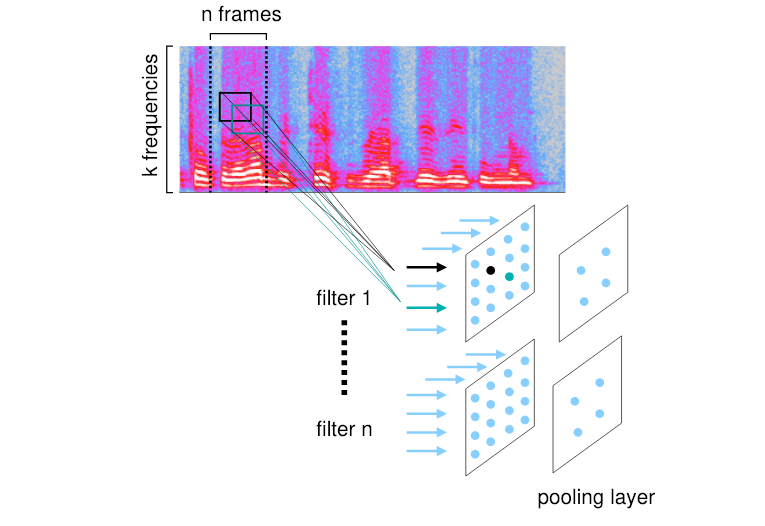
\includegraphics[width=0.7\textwidth]{figs/cnn}
\end{figure}
For a $2$D image, a layer can be written as
\begin{align}
\phi(z_{ij}) = \phi \Bigg [ \sum_{k, l} w_{kl} x_{(i-k)(i-l)}  \Bigg] \label{eq:cnn_conv}
\end{align}
where $w_{kl}$ represents the `weights' which control which filter operation is performed and defines an image filter.
\ix{Design Choices}A number of parameters control the form of CNN:
\begin{itemize}[]
	\item Depth: how many filters to apply. 
	\item Receptive Field: size of the filter applied i.e. height/width/depth. 
	\item Stride: spacing between filters i.e. how $i$ and $j$ vary in Eq. \ref{eq:cnn_conv}
	\item Dilation: `gaps' between filter elements. This allows a larger receptive field without an increase in parameters. 
	\item Zero-Padding: edges of images could be padded with zeroes. 
\end{itemize}
An\ix{Autoencoder}\marfig{figs/autoencoder}{} \emph{Autoencoder} is a type of feed-forward network which is trained to encode an input into a low dimension code layer and decode the low dimensional representation, reconstructing the original input. This can be used to de-noise data as well as perform non-linear feature extraction. The error function penalises the reconstruction error:
\begin{align}
E(\vect{\theta}) = \sum_{p=1}^n f(\vect{x}_p, \hat{\vect{x}_p})
\end{align}

\subsection*{Training \& Back-Propagation}
\ix{One-Hot Encoding}For classification tasks, class labels are \emph{one-hot} encoded into vectors. Denote the true class of data point $i$ as $y_i \in \lbrace \omega_1, \ldots, \omega_k \rbrace$. For each datapoint, there is a target vector, $\vect{t}_i$, meaning that $\altmathcal{D} = \lbrace (\vect{x}_1, \vect{t}_1), \ldots, (\vect{x}_N, \vect{t}_N)  \rbrace$. 
\begin{align}
	t_{ij} = \begin{cases}
	1\hspace{0.25cm} & y_i = \omega_j \\
	0\hspace{0.25cm} & \text{otherwise}
	\end{cases}
\end{align}
Two\ix{Training Criteria} typical training criteria for such tasks are: 
\begin{itemize}
	\item Least squares error
	\begin{align}
	E(\vect{\theta}) = \frac{1}{2} \sum_{i=1}^N || \altmathcal{F}(\vect{x}_i) - \vect{t}_i||_2^2
	\end{align}
	This training criteria can be applied directly to regression problems where $\vect{y}_i$ takes the place of $\vect{t}_i$. Minimisation of the least-squares error corresponds to the maximum-likelihood solution where the likelihood is Gaussian with a scaled identity covariance matrix. 
	\item Cross-Entropy:
	\begin{align}
	E(\vect{\theta}) = - \sum_{i=1}^N \sum_{j=1}^K t_{ij} \log(\altmathcal{F}(\vect{x}_i)_j)
	\end{align}
	Recalling the one-hot encoding employed, the cross-entropy error maximises the average output value for each class. Note that this error is not strictly positive. 
\end{itemize}
Note that the output layer activation function must be chosen to be appropriate e.g. when attempting to predict a non-negative quantity, the activation function must ensure that this is indeed the case. For example, when predicting the variance of a random variable, the activation layer could be exponential.

\emph{Mixture Density Neural Networks}\marfig{figs/mixture_density_network}{Mixture Density Neural Networks} are a mix between probabilistic models and neural networks. A mixture of $M$ Gaussians is predicted with a neural network used for the prior mixture proportions, the mixture means i.e. the mixture components. For each component $m$, the neural network outputs
\begin{align}
\vect{y}_m(\vect{x}_p) = \begin{bmatrix}
\altmathcal{F}^{c}_m(\vect{x}_p) \\
\altmathcal{F}^{\mu}_m(\vect{x}_p) \\
\altmathcal{F}^{\sigma}_m(\vect{x}_p) \\
\end{bmatrix}
\end{align}
The model is then optimised using maximum likelihood. Note: this is a general technique for performing regression with an arbitrary output density for each input data-point. 
\begin{align}
p(\vect{y}_p|\vect{x}_p, \vect{\theta}) = \sum_{m=1}^M \altmathcal{F}^{c}_m(\vect{x}_p) \altmathcal{N}(\vect{y}_p|\altmathcal{F}^{\mu}_m(\vect{x}_p), \altmathcal{F}^{\sigma}_m(\vect{x}_p) )
\end{align}
\ix{Gradient Descent}\emph{Gradient Descent} is a simplistic gradient descent algorithm used for optimisation if there is no closed form solution. 
\begin{align}
	\vect{\theta}^{(i+1)} = \vect{\theta}^{(i)} - \eta \frac{\partial E}{\partial \vect{\theta}}\Bigg|_{\vect{\theta}^{(i)}}
\end{align}
$\eta$ is known as the \emph{learning rate} and is a free parameter which can be difficult to choose. It is desired to avoid local minima. Note that the gradient of the error function is required. 

For a single layer perceptron\ix{Single Layer Perceptron Training} with some error function $E(\vect{\theta})$, the chain rule is used to compute derivatives throughout the network as follows
\begin{align}
\frac{\partial E(\vect{\theta})}{\partial w_i} = \frac{\partial E(\vect{\theta})}{\partial y(\vect{x})} \frac{\partial y(\vect{x})}{\partial z} \frac{\partial z}{\partial w_i}
\end{align} 
The gradient is composed of terms depending on the cost function (change of error with the network output),  the activation function (change of network output with activation function inputs) and the network weights (change of activation function inputs with input). Note that this requires that the activation function is smooth and can be differentiated. 

\ix{Deriving Back-Propagation - Notation} Consider a multi-layer perceptron with $d$-dimensional input data, $L$ hidden layers (and so $L+1$ layers in total), $N^{(k)}$ nodes in level $k$ and $K$ dimensional output. Denote the input to the $k$th layer as $\vect{x}^{(k)}$ and the `extended input'\ix{Extended Input} as $\tilde{\vect{x}}^{(k)} = \begin{bmatrix}
\vect{x}^{(k)} & 1
\end{bmatrix}^T$. $\vect{W}^{(k)}$ is the weight matrix of the $k$th layer and thus has dimension $N^{(k)} \times N^{(k+1)}$ by definition. Each row of the weight matrix defines a node in layer $k$. Similarly, the weight matrix can be extended to include the bias term $\tilde{\vect{W}}^{(k)} = \begin{bmatrix}
\vect{W}^{(k)} & \vect{b}^{(k)}
\end{bmatrix}$ where $\vect{b}^{(k)}$ is the $N^{(k)}$ length column vector of node biases. The target values for network training are denoted at $\vect{t}$. Then, the equations governing the behaviour of the multi-layer perception are
\begin{align}
\vect{x}^{(1)} &= \vect{x} \\
\vect{x}^{(k)} &= \vect{y}^{(k-1)}\ \text{ for } k=\lbrace{2, \ldots,(L+1)}\rbrace \\
\vect{z}^{(k)} &= \tilde{\vect{W}}^{(k)} \tilde{\vect{x}}^{(k)} \\
\vect{y}^{(k)} &= \phi(\vect{z}^{(k)}) \\
\vect{y}(\vect{x}) &= \vect{y}^{(L+1)}
\end{align}
We\ix{Deriving Back Propagation} need to calculate $\frac{\partial E}{\partial \tilde{W}^{(k)}_{ij}}$ for all layers. The chain rule gives
\begin{align}
\frac{\partial E}{\partial \tilde{W}^{(k)}_{ij}} = \underbrace{\frac{\partial E}{\partial z_{i}^{(k)}}}_{\delta_i^{(k)}} \underbrace{\frac{\partial z_i^{(k)}}{\partial \tilde{w}_{ij}^{(k)}}}_{\tilde{x}_j^{(k)}}
\end{align}
For the output node, the evaluation of $\delta_i$ is straightforward (the same as the single layer perceptron). \ix{Evaluating $\delta$ for hidden layers}For hidden layers, 
\begin{align}
\nonumber \delta_i^{(k)} &= \sum_m \frac{\partial E}{\partial z_m^{(k+1)}} \frac{\partial z_m^{(k+1)}}{\partial z_i^{(k)}} \\
&=  \sum_m \frac{\partial E}{\partial z_m^{(k+1)}} \frac{\partial y_i^{(k)}}{\partial z_i^{(k)}} \frac{\partial z_m^{(k+1)}}{\partial y_i^{(k)}} \label{eq:hidden_layer}
\end{align}
but $z_m^{(k+1)} = \sum_j \tilde{W}_{mj}^{(k)} y^{(k)}_j$ and $y_j^{(k)} = \phi(z_j^{(k)})$ (see above). Therefore, \textbf{for the sigmoidal activation function}
\begin{align}
\delta_i^{(k)} = y_i^{(k)} (1 - y_i^{(k)}) \sum_m \delta_{m}^{(k+1)} \tilde{W}_{mi}^{(k)}
\end{align}
In\ix{Matrix Formulation} matrix notation, 
\begin{align}
\frac{\partial E}{\partial \tilde{\vect{W}}^{(k)}} = \vect{\delta}^{k} (\tilde{\vect{x}}^{(k)})^T
\end{align}
Define the activation derivative matrix for layer $k$ as 
\begin{align}
\bm{\Lambda}^{(k)} = \begin{bmatrix}
\frac{\partial y_1^{(k)}}{\partial z_1^{(k)}} & \ldots & \frac{\partial y_{N^{(k)}}^{(k)}}{\partial z_1^{(k)}} \\
\vdots & \dots & \vdots \\
\frac{\partial y_1^{(k)}}{\partial z_{N^{(k)}}^{(k)}} & \ldots & \frac{\partial y_{N^{(k)}}^{(k)}}{\partial z_{N^{(k)}}^{(k)}}
\end{bmatrix}
\end{align}
Note that this is diagonal for most layers.  Eq. \ref{eq:hidden_layer} can be modified to include non-diagonal terms of the activation derivative matrix as follows
\begin{align}
 \nonumber \delta_i^{(k)} &=  \sum_m \underbrace{\frac{\partial E}{\partial z_m^{(k+1)}}}_{\delta_m^{(k+1)}} \sum_j \underbrace{\frac{\partial y_j^{(k)}}{\partial z_i^{(k)}}}_{\Lambda_{ij}^{(k)}} \underbrace{\frac{\partial z_m^{(k+1)}}{\partial y_j^{(k)}}}_{\tilde{W}^{(k+1)}_{mj}} \\
 &= \sum_{m, j} \Lambda_{ij}^{(k)} \tilde{W}^{(k+1)}_{mj} \delta_m^{(k+1)} \\
 \therefore\ \vect{\delta}^{(k)} &= \bm{\Lambda}^{(k)} (\vect{W}^{(k+1)})^T \vect{\delta}^{(k)+1}
\end{align}
Thus a matrix form for the back-propagation algorithm has been found.\ix{Back-Propagation - Initialisation} The initialisation of the backward recursion is from the output player. 
\begin{align}
\nonumber \vect{\delta}^{(L+1)} &= \frac{\partial E}{\partial \vect{z}^{(L+1)}} \\
&= \bm{\Lambda}^{(L+1)} \frac{\partial E}{\partial \vect{y}(\vect{x})}
\end{align}
Thus, the process to get the derivative involves propagating forwards $\vect{y}^{k}$ and $\vect{z}^{(k)}$, computing the gradient at the output layer and then propagating back $\vect{\delta}$, using this value to compute the desired derivative. 

\subsection*{Optimisation}
The gradient is calculated over all training samples; for large datasets, this is very slow. A simple modification is to use batch gradient descent where only a subset of the data is used to calculate the gradient. There is a compromise involved with choosing the size of the subset used as if too small, the gradient estimate is poor but the computation cost rises with subset size. \ix{Stochastic Gradient Descent}A modification is made to this algorithm; the order of the data presented for training is randomised and mini-batch updates (with random subsets) are used.

These\ix{Gradient Descent: Issues \& Solutions} algorithms have issues with stopping at local minima and handling `ravines'. A method of resolving this is by introducing \emph{Momentum}:
\begin{align}
\Delta \vect{\theta}^{(k)} = \eta \underbrace{\frac{\partial E}{\partial \vect{\theta}} \Bigg |_{\vect{\theta}^{(k)}}}_{\nabla_{\vect{\theta}} E } + \alpha \Delta \vect{\theta}^{(k-1)}
\end{align}
This serves to smooth parameter changes over iterations. Additionally, the learning rate can be modified to be a function of the iteration, $k$. A simple approach is to have a larger learning rate when the previous iteration decreases the cost function. 

Gradient\ix{Second-Order Approximation} descent only makes use of the first order derivative. A multi-dimensional Taylor expansion reads
\begin{align}
E(\vect{\theta}) = E(\vect{\theta}^{(k)}) + (\vect{\theta} - \vect{\theta}^{(k)}) \frac{\partial E}{\partial \vect{\theta}} \Bigg |_{\vect{\theta}^{(k)}} + \frac{1}{2} (\vect{\theta} - \vect{\theta}^{(k)})^T \vect{H}_{\vect{\theta}^{(k)}} (\vect{\theta} - \vect{\theta}^{(k)}) + \altmathcal{O}(\vect{\theta}^3)
\end{align}
where $\vect{H}_{\vect{\theta}^{(k)}}$ is the Hessian matrix of second derivatives. Taking derivatives and ignoring high order second order terms (valid when the error function is locally well approximated by a quadratic) gives
\begin{align}
\nabla_{\vect{\theta}} E(\vect{\theta}) \simeq \frac{\partial E}{\partial \vect{\theta}} \Bigg |_{\vect{\theta}^{(k)}} + \vect{H}_{\vect{\theta}^{(k)}} (\vect{\theta} - \vect{\theta}^{(k)})
\end{align} 
Equating this to zero gives
\begin{align}
\Delta \vect{\theta}^{(k)} = - \vect{H}^{-1}_{\vect{\theta}^{(k)}} \frac{\partial E}{\partial \vect{\theta}} \Bigg |_{\vect{\theta}^{(k)}}
\end{align}
Note that care must be taken to ensure that a minimum in the cost function is found (i.e. the Hessian matrix is positive semi-definite). Whilst\ix{Problems with Second-Order Approaches} in theory this works, there are a number of issues in practice:
\begin{enumerate}
	\item The evaluation of the Hessian can be computationally challenging as $\altmathcal{O}(N^2)$ parameters must be accumulated for each sample. 
	\item At each iteration, the Hessian must be inverted - this is an $\altmathcal{O}(N^3)$ operation. 
	\item There is no guarantee that the step leads to a minimum; a maximum or saddle point could be reached instead. 
	\item If the surface is poorly locally approximated by a quadratic, the step sizes may be too large and the optimisation technique will be unstable. 
\end{enumerate}

A\ix{QuickProp} technique known as \emph{QuickProp} assumes that the error surface is quadratic in nature with a diagonal Hessian, allowing each weight to be treated independently. Denote the estimate for $\theta$ as time-step $\tau$ as $\theta^{\tau}$
\begin{align}
E(\theta, \hat{\theta}) &\simeq E(\hat{\theta}) + b(\theta - \hat{\theta}) + a(\theta - \hat{\theta})^2 \\
g^{\tau'}&= \frac{\partial E(\theta, \hat{\theta}^{\tau})}{\partial \theta} \Big |_{\theta = \theta^{\tau'}} \simeq b + 2a(\theta^{\tau'} - \theta^{\tau} )
\end{align}
It is desired that the gradient be zero after the next update. Thus:
\begin{align}
g^{\tau - 1} &\simeq b + 2a(\theta^{\tau - 1} - \theta^\tau) = b - 2a \Delta \theta^{\tau - 1} \\
g^{\tau} &\simeq b \\
g^{\tau + 1} &\simeq b + 2a \Delta \theta^{\tau}
\end{align}
Rearranging and solving for $g^{\tau + 1} = 0$ yields:
\begin{align}
\Delta \theta^{\tau} = \frac{g^{\tau} \cdot \Delta \theta^{\tau-1}}{g^{\tau - 1} - g^{\tau}}
\end{align}

Generalisation\ix{Regularisation} performance is essential. Regularisation techniques prevent \emph{overfitting} which is when training data performance increases whilst generalisation performance decreases (i.e. the network fits to the noise in the dataset). \emph{Regularisation} is used to address this. Forms of regularisation include
\begin{itemize}
	\item Early stopping - do not train the network to convergence but rather stop early.
	\item Constraining parameter size (effectively placing a zero `prior' on the network parameters) i.e. modify the cost function as follows
	\begin{align}
	\tilde{E}(\vect{\theta}) = E(\vect{\theta}) + \nu \cdot \frac{1}{2} \sum_{l, i, j} (w_{ij}^{(l)})^2 
	\end{align}
	this is incredibly simple to include in gradient descent optimisation. 
	\item \emph{Dropout}\ix{Dropout}: a random proportion of network nodes are `deactivated' (relevant terms are excluded from the back-propagation algorithm) and model parameters are updated during each step of the training process. \textbf{This prevents a single node specialisation to a task} and thus improves generalisation. 	
\end{itemize}
Data features have different dynamic ranges. \ix{Weight Initialisation}For example, one feature could be measured in $\mu m$ whilst another is measured in $km$. This affects the relative `importance' of features during the training process. \ix{Data Preprocessing} Data whitening is often employed to prevent gradients from being dominated by one term only and ensures that each feature as the same mean and variance. 
\begin{align}
\tilde{x}_{ni} &= \frac{x_{ni} - \mu_i }{\sigma_i} \\\text{ where } \mu_i &= \sum_{n=1}^{N} \frac{x_{ni}}{N} \\ \sigma_i^2 &= \frac{1}{N} \sum_{n=1}^{N} (x_{ni} - \mu_i)^2 
\end{align}

The\ix{Network Initialisation: Weight Parameters} gradient descent algorithm requires an initialisation for the weights. We need to worry about both vanishing gradients (gradients going to zero resulting in no parameter updates) and exploding gradients (derivatives getting very large and causing saturation). Whilst it is not possible to guarantee a good starting point, a Gaussian random initialisation passed through a sigmoid non-linearity can work well. \textbf{Note: } we need to be careful about the initialisation of the weights - if we choose them too large, passing data through the sigmoid will end up with saturated sigmoids. In regions where the sigmoid has saturated, the gradient will be small because the gradients of the activation functions themselves are small in these regions; this the variance should be chosen to avoid these small gradients. 

To avoid the problems of vanishing and exploding gradients, the input and output variance should be the same. This leads to the \emph{Xavier Initialisation}\ix{Xavier Initialisation} where $\text{var}(w_{ij}^{(l)}) = \frac{1}{N^{(l-1)}}$. This can be justified by assuming linear activation functions $\vect{y} = \vect{Wx}$, that all weights are independent and everything has zero mean. Then
\begin{align}
\text{var}(y_i^{k}) = \text{var}\Bigg( \sum_{j} W_{ij}x_j \Bigg) = N^{(k-1)} \text{var}(w_{ij}) \text{var}(x_j)
\end{align} 

\emph{Batch Normalisation}\ix{Batch Normalisation} processes the output of each layer with a normalisation term that varies as the system trains in an attempt to ensure values remain in the linear region. The output of each layer is normalised by considering only a batch of the data meaning that each normalisation term is only a noisy estimate of the true term. At test time, the normalisation constant is found by considering taking the expectation over a large number of different batches (from the training set).

\section{Deep Learning for Sequence Data}
The previous deep learning techniques that we have seen have assumed that the input data is a fixed size. We will now focus on data which is of variable length, the key requirement being the sharing of model parameters to let us handle variable length inputs. There are a number of specific tasks that can be performed for such data, which will considered each in turn. Note that $\vect{x}_{1:T}$ denotes $\lbrace \vect{x}_1, \ldots, \vect{x}_T \rbrace$.

\subsection{Sequence (Input, Output) Pairing}
Sequence (input, output) pairing produces the sequence $\lbrace (\vect{x}_1, \vect{y}_1), \ldots, (\vect{x}_T, \vect{y}_T) \rbrace$ from the input sequence $\vect{x}_{1:T}$. \ix{Example Task- PoS Tagging} An example task of this type is \emph{part of speech tagging} where each word in the text sequence is tagged with a particular part of speech e.g. nouns, verbs, adverbs (though typically the tags are more advanced than this). This is a challenging problem as individual words are ambiguous and they function depends on their context within a sentence. 

\marfig{figs/rnns}{Recurrent Neural Networks} \emph{Recurrent Neural Networks} are a family of neural networks designed to process sequential data. Variable length sequences are dealt with by introducing an approximate \emph{history vector}, $\vect{h}_t$, which models the history of observations. 
\begin{align}
\altmathcal{F}(\vect{x}_{1:t}) = \altmathcal{F}(\vect{x}_t, \vect{x}_{1:(t-1)}) \simeq \altmathcal{F}(\vect{x}_t, \vect{h}_{t-1}) \simeq \altmathcal{F}(\vect{h}_t)
\end{align}
The history vector is updated using a neural network. 
\begin{align}
\vect{h}_t = \altmathcal{F}^{(h)} (\vect{W}_h^f\vect{x}_t + \vect{W}_h^r\vect{h}_{t-1} + \vect{b}_h)
\end{align}
Note that the $\vect{W}$ matrices are simple linear transformations of the input and history vector at each point. Additionally, the output is determined by an additional neural network.
\begin{align}
y(\vect{x}_{1:t}) = \altmathcal{F}^{(y)}(\vect{W}_y \vect{h}_t + \vect{b}_y)
\end{align}
The network has causal memory encoding into the history vector. There are two main advantages of this structure:
\begin{enumerate}
	\item Regardless of the sequence length, the learned model always has the same input size as it is specified in terms of the transition from state to state. 
	\item It is possible to use the same transition functions at every time step, corresponding to one shared set of weights. 
\end{enumerate}
This means that a single model can be learnt which operates on all time-steps for variable sequence lengths. 

\marfig{figs/jordan_network}{}This topology is known as the \emph{Elman Network}. An alternative topology is known as the \emph{Jordan Network} in which the history vector remembers the unobserved output sequence, $\vect{y}_{1:T}$.

\begin{align}
\altmathcal{F}(\vect{x}_{1:t}, \vect{y}_{1:t-1}) \simeq \altmathcal{F}(\vect{x}_{t}, \vect{y}_{1:t-1}) \simeq \altmathcal{F}(\vect{x}_{1:t}, \vect{h}_{t-1}) \simeq \altmathcal{F}(\vect{h}_t)
\end{align}

\marfig{figs/bi-rnn}{}Alternatively, \emph{Bi-Directional RNNs} may be used in which the complete observation sequence is used:
\begin{align}
\altmathcal{F}_t(\vect{x}_{1:T}) = \altmathcal{F}_t(\vect{x}_{1:t}, \vect{x}_{t+1:T}) \simeq \altmathcal{F}_t(\vect{h}_t, \tilde{\vect{h}}_t)
\end{align} 

Network gating is a technique which creates paths through the network with derivatives that neither vanish nor explode. 

\marfig{figs/GRU}{}The equations for the \emph{Gated Recurrent Unit} are:
\begin{align}
\vect{i}_f &= \sigma(\vect{W}_{f}^{f} \vect{x}_t + \vect{W}_{f}^{h} \vect{h}_t + \vect{b}_f) \hspace{1cm} \text{(forget gate)} \\
\vect{i}_o &= \sigma(\vect{W}_{o}^{f} \vect{x}_t + \vect{W}_{o}^{h} \vect{h}_t + \vect{b}_o) \hspace{1cm} \text{(output gate)} \\
\vect{h}_t &= \vect{i}_0 \odot \vect{h}_{t-1} + (1 - \vect{i}_0) \odot \altmathcal{F}\ \Big( \vect{W}^{f}_{y} \vect{x_t} +  \vect{W}^{h}_{y} (\vect{i}_f \odot \vect{h}_{t-1}) + \vect{b}_y) \Big)
\end{align}
The forget and output gate can individually ignore parts of the history vector (given the state value). The output gate affects every dimension, allowing the new history to be purely the old history vector (at one extreme of the sigmoid) or replacing it with the new target state value. The forget gate controls which parts of the state are used to compute the next target state.

\marfig{figs/LSTM}{Long-Short Term Memory Units}\emph{Long-Short Term Memory Units (LSTMs)} are more complex than GRUs. The equations underpinning the LSTM are:
\begin{align}
\vect{i}_f &= \sigma\Big( \vect{W}_{f}^{f}\vect{x}_t + \vect{W}_{f}^{h} \vect{h}_{t-1} + \vect{W}_{f}^{m} \vect{c}_{t-1} + \vect{b}_{f}  \Big) \\
\vect{i}_i &= \sigma\Big( \vect{W}_{f}^{i}\vect{x}_t + \vect{W}_{i}^{h} \vect{h}_{t-1} + \vect{W}_{i}^{m} \vect{c}_{t-1} + \vect{b}_{i}  \Big) \\
\vect{i}_o &= \sigma\Big( \vect{W}_{f}^{o}\vect{x}_t + \vect{W}_{o}^{h} \vect{h}_{t-1} + \vect{W}_{o}^{m} \vect{c}_{t} + \vect{b}_{o}  \Big) \\
\vect{c}_t &= \vect{i}_f \odot \vect{c}_{t-1} + \vect{i}_i \odot \altmathcal{F}^{m}\ (\vect{W}_{c}^{f} \vect{x}_t + \vect{W}_{c}^{h} \vect{h}_{t-1} + \vect{b}_c ) \\
\vect{h}_t &= \vect{i}_o \odot \altmathcal{F}^h (\vect{c}_t)
\end{align}
The LSTM includes a memory cell with diagonal weight matrices. The self-loop of the memory cell is controlled by a forget gate unit and the update is also dependent on an input gate unit. The output gate unit allows the output of the LSTM to be shut-off. The LSTM is able to learn long-term dependencies more easily than simply recurrent architectures. 

\marfig{figs/highway_con}{Highway Connections} \emph{Highway Connections} gate the output of the node and combine them with the output from the previous layer:
\begin{align}
\vect{i}_h &= \sigma (\vect{W}^{f}_{i} \vect{x}_t + \vect{W}^{h}_{i}\vect{h}_{t-1} + \vect{b}_i) \\
\vect{h}_t &= \vect{i}_h \odot \altmathcal{F} (\vect{W}^{f}_{h} \vect{x}_t + \vect{W}^{h}_{h} \vect{h}_{t-1} + \vect{b}_h) + (1 - \vect{i}_h) \odot \vect{x}_t
\end{align}
Note that the node could be anything e.g. an LSTM, a GRU, etc.

\subsection{Input Sequence to Target}
A typical example of this sort of task is sentiment analysis given a sequence of words. 

\ix{Averaging Approach}A simple method of performing this sort of task would be averaging as follows:
\begin{align}
\vect{h}_t &= \altmathcal{F}_1(\vect{x}_t) \\
\vect{c} &= \frac{1}{T} \sum_{t} \vect{h}_t \\
\tilde{\vect{h}} &= \altmathcal{F}_2(\vect{c}) \\
\vect{y} &= \altmathcal{F}_3(\tilde{\vect{h}})
\end{align}
Note that several transformations are required; the first transformation is into a space where averages can be taken meaningfully. The average itself, $\vect{c}$, is then transformed into a space in which classification can occur. The network can then simply be trained 

\marfig{figs/sequence_embedding}{Sequence Embedding}An alternative is \emph{Sequence Embedding} in which the final history vector is used to perform the task. This is able to handle variable length input sequences, but tends to be biased towards later inputs. A simple remedy is to used bi-directional information, and the final output is produced using both the forwards and reverse history vector. 

\marfig{figs/attention}{Attention Mechanism}The \emph{Attention Mechanism} is the extension of the averaging approach, altering the average to be a function of some key, $\vect{k}$. 
\begin{align}
c &= \sum_{t} \alpha_t \vect{h}_t \\
\alpha_t &= \frac{\exp (e_t)}{\sum_i \exp (e_i)} \\ 
\tilde{\vect{h}} &= \altmathcal{F}_1(\vect{k}) \\
e_t &= \altmathcal{F}_2(\vect{h}_t, \tilde{\vect{h}})
\end{align}
$\alpha_t$ is a probability mass function over the input sequence. Note that it is vital to choose appropriate $\vect{k}$ and $\altmathcal{F}_2(\cdot, \cdot)$ which relates the key to the observation. \ix{Typical Attention Forms}Typical forms of attention include:
\begin{enumerate}
	\item Dot-product attention:
	\begin{align}
	e_t = \vect{h}_t^{T} \vect{W}_{xk} \tilde{\vect{h}}
	\end{align}
	This has parameters $\vect{W}_{xk}$.
	
	\item Additive attention:
	\begin{align}
	e_t = \vect{w}^{T} \tanh (\vect{W}_x \vect{h}_t + \vect{W}_k \tilde{\vect{h}})
	\end{align}
	This has parameters $\vect{w}, \vect{W}_x$ and $\vect{W}_k$. 
\end{enumerate}
For example, a question and response task could be solved by encoding both the question and document both forwards and backwards, using a suitable the attention mechanism with the key chosen to be the question encoding. Attention mechanisms are interpretable and the most relevant word in a document can clearly be examined. 

\subsection{Sequence to Sequence}
A typical sequence-to-sequence machine learning task would be translating a word sequence into another language. 

\ix{Encoder-Decoder Sequence Models}An encoder-decoder sequence models trains a model from $\vect{x}_{1:L}$ (e.g. source language) and $\vect{y}_{1:K}$ (e.g. target language): \marfig{figs/rnn_encode_decode}{}
\begin{align}
p(\vect{y}_{1:k} | \vect{x}_{1:L}) &= \prod_{i=1}^K p(\vect{y_i} | \vect{y}_{1:i-1}, \vect{x}_{1:L}) \\
&\simeq \prod_{i=1}^K p(\vect{y_i} | \vect{y}_{i-1}, \tilde{\vect{h}}_{i-1}, \vect{c} )
\end{align}
i.e. $\vect{x}_{1:L}$ must be mapped to a \textbf{fixed-length} vector, $\vect{c} = \phi(\vect{x}_{1:L})$. One form is to use the hidden unit from an RNN/LSTM/GRU i.e. $\vect{c} = \vect{h}_{L}$. Depending on the context is global through $\vect{c}$, which may be limiting. 

An attention based model\marfig{figs/attention_ss}{Attention-Based Model} introduces dependence on locality:
\begin{align}
p(\vect{y}_{1:K} | \vect{x}_{1:L}) &\simeq \prod_{i=1}^{K} p(\vect{y}_i | \vect{y}_{i-1}, \tilde{\vect{h}}_{i-1}, \vect{c}_i) \simeq \prod_{i=1}^{K} p(\vect{y}_i | \tilde{\vect{h}}_i) \\
\vect{c}_i &= \sum_{\tau = 1}^{L} \alpha_{i, \tau} \vect{h_\tau} \\
\alpha_{i\tau} &= \frac{\exp(e_{i\tau})}{\sum_{j=1}^{L} \exp(e_{ij})} \\
e_{i\tau} = &\altmathcal{F}(\tilde{\vect{h}}_{i-1}, \vect{h}_\tau)
\end{align}
The decoder part of the model is similar to the Jordan network, and the history vector encodes the outputs \textbf{and} context histories i.e.
\begin{align}
p(w_i| \hat{w}_{0:i-1}, w_{1:L}^{(s)}) \simeq p(w_i| \hat{\vect{y}}_{0:i-1}, \vect{c}_{1:i}^{(s)}) \simeq p(w_i| \tilde{\vect{h}}_i)
\end{align}
where each $\vect{x}$ represents embedding of a source language word, $\vect{c}_i$ is the context information for word $i$, $\hat{w}_i$ is the generated target language word at time $i$ and $\hat{\vect{y}}_i$ is the embedding of the generated word $\hat{w}_i$. 

\ix{Performing Inference} First, the source language word sequence is encoded i.e. $w_{1:L}^{(s)} \rightarrow \vect{x}_{1:L}$. Then, to generate word $\hat{w}_i$:
\begin{enumerate}
\item Embed the previous word: $\hat{w}_{i-1} \rightarrow \vect{y}_{i-1}$. 
\item Compute context information using key.
\item Generate new history vector: $\tilde{\vect{h}}_i = \altmathcal{F}(\tilde{\vect{h}}_{i-1}, \hat{\vect{y}}_{i-1}, \vect{c}_i)$.
\item Use $\tilde{\vect{h}}_i$ to compute $P(w_i |\tilde{\vect{h}}_i)$, which is then sampled from. 
\end{enumerate}
An issue with this approach is that the system can go off-track, and the system isn't very robust to model history errors. 

\subsection{Single Input to Sequence}
An example task would be to caption images.\marfig{figs/image_caption}{Image Captioning} In this case, the image would be encoded as a vector using e.g. a deep convolutional network, generating an output vector. This is fed into a recurrent network which generates a caption. Typically trained on example image captions. This system is trained end-to-end, minimising the need for human expertise. The encoder output need not be interpretable.  

\section{Variational Autoencoders}
A \emph{Variational Autoencoder}\ix{VAE} is a rich, latent variable model of the form:
\begin{align}
p(\vect{z}) &= \altmathcal{N}(\vect{z}| 0, \vect{I}) \label{eq:vae_1}\\
p(\vect{x}|\vect{z}, \vect{\lambda}) &= \altmathcal{N}(\vect{x})| \altmathcal{F}(\vect{z}; \vect{\lambda}), \sigma^2 \vect{I} )) \label{eq:vae_2}
\end{align}
The idea is to use a deep neural network to learn the mapping between the latent and mean observation. However, the log-likelihood cannot be computed for inference, and it's gradients can also not be computed. Thus, variational approaches are applied. 

\subsection{Variational EM}
In the EM algorithm, an auxiliary function is maximised rather than the log-likelihood:
\begin{align}
\vect{\lambda}^{(k+1)} = \arg \max_{\vect{\lambda}} \int p(\vect{z} | \vect{x}, \vect{\lambda}^{(k)}) \log p(\vect{x}, \vect{z}| \vect{\lambda}) d\vect{z}
\end{align}
This workers because in many models (e.g. factor analysis), the expected value of the log joint is simple, and often a function of the posterior moments of the latent.

However\ix{Log Likelihood}, we now return to the log-likelihood:
\begin{align}
\altmathcal{L}(\vect{\lambda}) &= \log p(\vect{x}| \vect{\lambda}) \nonumber\\
&= \int p(\vect{z}| \vect{x},  \vect{\lambda}) \log p(\vect{x}| \vect{\lambda}) d\vect{z} \nonumber \\
&=  \int p(\vect{z}| \vect{x},  \vect{\lambda}) \log \frac{p(\vect{x}| \vect{\lambda}) p(\vect{z}| \vect{x},  \vect{\lambda})}{p(\vect{z}| \vect{x},  \vect{\lambda})} d\vect{z} \nonumber \\ 
&= \mathbb{E}_{p(\vect{z}| \vect{x},  \vect{\lambda})} \Big[ \log \frac{p(\vect{z}, \vect{x}|  \vect{\lambda})}{p(\vect{z}| \vect{x},  \vect{\lambda})} \Big]
\end{align}
\ix{Why is this difficult?}In order to evaluate this, the posterior over the latent variables needs to be calculated. Consider some proposal distribution, $q(\vect{z}| \vect{\lambda})$:
\begin{align}
\altmathcal{L}(\vect{\lambda}) &= \log p(\vect{x}| \vect{\lambda}) \nonumber\\
&= \int q(\vect{z}| \vect{\lambda})) \log p(\vect{x}| \vect{\lambda}) d\vect{z} \nonumber \\
&=  \int q(\vect{z}| \vect{\lambda}) \log \frac{p(\vect{x}| \vect{\lambda}) p(\vect{z}| \vect{x},  \vect{\lambda})}{p(\vect{z}| \vect{x},  \vect{\lambda})} d\vect{z} \nonumber \\ 
&= \mathbb{E}_{q(\vect{z}| \vect{\lambda})} \Big[ \log \frac{p(\vect{z}, \vect{x},  \vect{\lambda})}{p(\vect{z}| \vect{x},  \vect{\lambda})} \Big] \nonumber \\
&= \underbrace{\mathbb{E}_{q(\vect{z}| \vect{\lambda})} \Big[ \log \frac{p(\vect{x}, \vect{z}|  \vect{\lambda})}{q(\vect{z}| \vect{\lambda})} \Big]}_{\altmathcal{F}(q, \vect{\lambda})} + \underbrace{\altmathcal{KL}(q(\vect{z}| \vect{\lambda}) || p(\vect{z}| \vect{x},  \vect{\lambda}))}_{\geq 0}
\end{align}
$\altmathcal{F}(q , \vect{\lambda})$ is a lower bound on the free-energy, and equality is reached when $q(\vect{z}| \vect{\lambda}) = p(\vect{z}| \vect{x}, \vect{\lambda})$. \ix{Steps}The EM algorithm initialises q as the posterior for some parameter settings, $q(\vect{z}| \vect{\lambda}) = p(\vect{z}| \vect{x}, \hat{\vect{\lambda}})$, and then repeatedly:
\begin{enumerate}
	\item (M-Step): Maximise $\altmathcal{F}(q , \vect{\lambda})$ with respect to $\vect{\lambda}$, fixing the current proposal distribution. This effective maximises a lower bound of the log-likelihood. 
	\item (E-Step): Maximise $\altmathcal{F}(q , \vect{\lambda})$ with respect to $q$ i.e. set $q(\vect{z}| \vect{\lambda}) = p(\vect{z}| \vect{x}, \vect{\lambda})$. 
\end{enumerate}
\ix{Lyapunov Function for EM}The log-likelihood is a \emph{Lyapunov} function:
\begin{align}
\altmathcal{L}(\vect{\lambda}^{(k)}) \stackrel{\text{E Step}}{=} \altmathcal{F}(q(\vect{z}| \vect{\lambda}^{(k)}) , \vect{\lambda}^{(k)}) \stackrel{\text{M Step}}{\leq} \altmathcal{F}(q(\vect{z}| \vect{\lambda}^{(k)}) , \vect{\lambda}^{(k+1)}) \leq \altmathcal{L}(\vect{\lambda}^{(k+1})
\end{align}
Each iteration is thus guaranteed to not decrease the likelihood and a local maximum of the likelihood is found. The exact solution found depends on the initial parameters. 

\ix{General EM} However, we may not be able to calculate the posterior depending on our model, and thus \textbf{in general}, 
\begin{align}
\altmathcal{L}(\vect{\lambda}^{(k)}) \stackrel{\text{in general}}{\geq} \altmathcal{F}(q(\vect{z}| \vect{\lambda}^{(k)}) , \vect{\lambda}^{(k)}) \stackrel{\text{M Step}}{\leq} \altmathcal{F}(q(\vect{z}| \vect{\lambda}^{(k)}) , \vect{\lambda}^{(k+1)}) \leq \altmathcal{L}(\vect{\lambda}^{(k+1})
\end{align}
meaning that there is no guarantee of improving the likelihood after each iteration. \ix{Mean Field}A standard approximation used is the mean-field approximation:
\begin{align}
q(\vect{z}| \vect{\lambda}) = \prod_{i=1}^{N} q_i(z_i| \vect{\lambda})
\end{align}
\subsection{Variational Autoencoders}
Recall the equations governing the VAES (Equations \ref{eq:vae_1} and \ref{eq:vae_2}). The likehood of a datapoint is given by:
\begin{align}
p(\vect{x}|\vect{\lambda}) &=\int p(\vect{x}| \vect{z}, \vect{\lambda}) p(\vect{z})\ d\vect{z} \nonumber \\
&= \int \altmathcal{N}(\vect{x}| \vect{f}(\vect{z}| \vect{\lambda}), \sigma^2 \vect{I}) \altmathcal{N}(\vect{z}| \vect{0}, \vect{I})\ d\vect{z} 
\end{align}
This integral cannot be computed; $\vect{f}(\vect{z}| \vect{\lambda})$ is a non-linear function. 

\ix{Variational EM}We could use a variational EM maximisation, maximising the free energy, $\altmathcal{F}(q, \vect{\lambda})$ by alternating maximisations over $\vect{\lambda}$ and $q$. Appropriate forms of the proposal distribution are important, and they influence how tight the lower bound is for the optimisation. However, this is not usually possible for deep learning. Please note that $\tilde{\vect{\lambda}}$ represents the parameters of the proposal distribution (i.e. the encoder) and $\vect{\lambda}$ represents the parameters of the decoder.

\ix{Applying Gradient Descent}The gradient of the likelihood is approximated using the gradient of the lower bound:
\begin{align}
\nabla \altmathcal{L}(\vect{\lambda}) &\simeq \nabla \Bigg( \mathbb{E}_{q(\vect{z}| \tilde{\vect{\lambda}})} \Big[ \log \frac{p(\vect{x}, \vect{z}|  \vect{\lambda})}{q(\vect{z}| \tilde{\vect{\lambda}})} \Big] \Bigg) \nonumber \\
&=  \nabla \Bigg( \mathbb{E}_{q(\vect{z}| \tilde{\vect{\lambda}})} [ \log p(\vect{x}| \vect{z}, \vect{\lambda} )] +  \mathbb{E}_{q(\vect{z}| \tilde{\vect{\lambda}})} \Big [ \log \frac{p(\vect{z})}{q(\vect{z}| \tilde{\vect{\lambda}})} ) \Big] \Bigg)
\end{align}
A density network is used as the variational approximation, introducing a dependence on $\vect{x}$:
\begin{align}
	q(\vect{z}| \tilde{\vect{\lambda}}) \rightarrow q(\vect{z}| \vect{x}, \tilde{\vect{\lambda}}) = \altmathcal{N}(\vect{z}| \bm{\altmathcal{F}}_\mu(\vect{x}| \tilde{\vect{\lambda}}), \bm{\altmathcal{F}}_\Sigma(\vect{x}| \tilde{\vect{\lambda}}))
\end{align}
This is the encoder part of the network. The likelihood can now be re-written as:
\begin{align}
\altmathcal{L}(\vect{\lambda}) &= \mathbb{E}_{q(\vect{z}| \vect{x}, \tilde{\vect{\lambda}})} \Big[ \log \frac{p(\vect{z}, \vect{x},  \vect{\lambda})}{p(\vect{z}| \vect{x},  \vect{\lambda})} \Big] \nonumber \\
&= \mathbb{E}_{q(\vect{z}| \vect{x}, \tilde{\vect{\lambda}})} \Bigg \lbrace \underbrace{\log \frac{q(\vect{z}| \vect{x}, \tilde{\vect{\lambda})}}{p(\vect{z}| \vect{x}, \vect{\lambda})}}_{\text{error}}  + \underbrace{\log p(\vect{x}| \vect{z}, \vect{\lambda})}_{\text{decoding}} + \underbrace{\log \frac{p(\vect{z})}{q(\vect{z}| \vect{x}, \tilde{\vect{\lambda})}}}_{\text{encoding}}   \Bigg \rbrace
\end{align}
The error terms captures the difference between the likelihood and the free energy. Returning to the gradient of the lower bound, \ix{Rewriting and interpreting the likelihood}the dependence on $\vect{x}$ is now included:
\begin{align}
\nabla \altmathcal{L}(\vect{\lambda}) =  \nabla \Bigg( \mathbb{E}_{q(\vect{z}| \vect{x}, \tilde{\vect{\lambda}})} [ \log p(\vect{x}| \vect{z}, \vect{\lambda} )] +  \mathbb{E}_{q(\vect{z}| \vect{x}, \tilde{\vect{\lambda}})} \Big [ \log \frac{p(\vect{z})}{q(\vect{z}| \vect{x}, \tilde{\vect{\lambda}})} ) \Big] \Bigg)
\end{align}
The first term is difficult as the expectations of highly non-linear functions must be computed. Note that this term is a function of both $\vect{\lambda}$ and $\tilde{\vect{\lambda}}$ The second term is however easy to calculate as it is the KL divergence between Gaussians which has a simple closed-form solution. 

\ix{Using Monte-Carlo} Monte Carlo is used to evaluate the first term:
\begin{align}
\mathbb{E}_{q(\vect{z}| \vect{x}, \tilde{\vect{\lambda}})} [ \log p(\vect{x}| \vect{z}, \vect{\lambda} )] \simeq \frac{1}{N} \sum_{i=1}^N \log p(\vect{x}| \vect{z}^{(i)}, \vect{\lambda}) \text{ with } \vect{z}^{(i)} \sim q(\vect{z}| \vect{x}, \tilde{\vect{\lambda}})
\end{align}
Samples can be drawn easily since $q(\vect{z}| \vect{x}, \tilde{\vect{\lambda}})$ is Gaussian. However, this is directly using samples from $q(\vect{z}| \vect{x}, \tilde{\vect{\lambda}})$ and it does not allow gradients for $\tilde{\vect{\lambda}}$ to be calculated. 

\ix{Reparameterisation Trick}The reparameterisation trick solves this by noting that:
\begin{align}
\vect{z}^{(i)} = \bm{\altmathcal{F}}_\mu(\vect{x}| \tilde{\vect{\lambda}}) + \bm{\altmathcal{F}}_\Sigma(\vect{x}| \tilde{\vect{\lambda}})^{1/2} \vect{e}^{(i)} \text{ with }\vect{e}^{(i)} \sim \altmathcal{N}(\vect{0}, \vect{I})
\end{align}

\section{Ensemble Methods}
\ix{Simple Binary Classification} Consider an ensemble of binary classifiers with \textbf{independent} error probability, $p_e$, with overall classification performing using majority voting. The probability that such a classifier makes an error is:\marfig{figs/ensemble}{}
\begin{align}
\mathbb{P}(\text{error}) = \sum_{i={\frac{N+1}{2}}}^N \begin{pmatrix}
N \\ i
\end{pmatrix} p_e^i (1-p_e)^{N-1}
\end{align}
Consider an ensemble of discriminative, probabilistic classifiers. Extended the ensemble method approach, the decision rule becomes\ix{Decision Rule}:
\begin{align}
\hat{\omega} = \arg \max_{\omega} \Bigg \lbrace \sum_{\altmathcal{M}} \int \underbrace{P(\omega| \vect{x}^*, \vect{\theta}, \altmathcal{M})}_{\text{predictive | params}}\ \overbrace{p(\vect{\theta}| \altmathcal{M}, \altmathcal{D})}^{\text{posterior}}\ \underbrace{P(\altmathcal{M}| \altmathcal{D})}_{\text{posterior over models}}\ d\vect{\theta}  \Bigg \rbrace
\end{align}
$\altmathcal{M}$ specifies a model topology, and $\vect{\theta}$ are the parameters given that topology. This is a highly complex distribution, so we resort to Monte Carlo. 
\begin{align}
\hat{\omega} &= \arg \max_{\omega} \Big \lbrace \frac{1}{N} \sum_{j=1}^N P(\omega | \vect{x}^*, \altmathcal{M}^{(j)}) \Bigg \rbrace \nonumber \text{ with } \altmathcal{M}^{(i)} \sim p(\vect{\theta}, \altmathcal{M}|\altmathcal{D} )\\
\altmathcal{E} &= \Big \lbrace \altmathcal{M}^{(1)}, \ldots, \altmathcal{M}^{(N)} \Big \rbrace
\end{align}
However, the posterior $p(\vect{\theta}, \altmathcal{M}|\altmathcal{D})$ is incredibly complicated, and it is difficult to efficiently sample over it, especially over model topologies. Most of the approaches for ensemble methods are practical without significant links to theoretical sampling. 

Practical ensemble methods:
\begin{itemize}
	\item \ix{Bagging}One such procedure is \emph{Bagging} in which a subset of the data, $\tilde{\altmathcal{D}} \subset \altmathcal{D}$, $|\tilde{\altmathcal{D}}| = N$, is sampled (with or without replacement). The model is trained on $\tilde{\altmathcal{D}}$, and this is repeated until the desired ensemble size is generated.  
	
	\item \ix{Dropout}With dropout, random nodes are deactivated during each step of training according to some probability, which acts as regularisation, preventing one path becoming too specialised. In effect, we are sharing weights between a large number of models, and to compute the overall output, we de-weight weights by the inverse of the drop-out rate. This is approximately equivalent to computing the geometric mean of each sub-network.  \textbf{Using this method, we can train an ensemble using one network only}. 
	
	\item \ix{Random Network Initialisation}A simple alternative is to randomly initialise network parameters for a given network topology according to some prior distribution. Each member of the ensemble is then found by training the network from this initialisation, meaning that each ensemble method will be at a local optimum. 
	
	\item\ix{Adhoc Models}Another simple approach is to select different configurations (e.g. numbers and sizes of layers, nature of activation function and nature of the targets), then manually sampling from the `configuration posterior', with each system trained to a local optimum. This uses expert knowledge to improve synergies between different models in the ensemble. 
\end{itemize}

\ix{Posterior Combination}The simplest approach to posterior combination is to average the class posteriors from the ensemble:
\begin{align}
P(\omega | \vect{x}^*, \altmathcal{E}) = \frac{1}{N} \sum_{i} P(\omega | \vect{x}^*, \altmathcal{M}^{(i)}) 
\end{align}
However, this requires all models in the ensemble to be evaluated and stored for each test point. 

\ix{Teacher Student Training}Recall the standard cross entropy training criterion for classification with $\altmathcal{D} = \lbrace (x_i, y_i)\rbrace$ and $ y_i \in \lbrace \omega_1, \ldots, \omega_K \rbrace$.
\begin{align}
\altmathcal{L}_{\text{ce}} = -\sum_{i=1}^n \sum_{\omega} \delta(y_i, \omega) \log P(\omega| \vect{x_i}, \altmathcal{M})
\end{align}
This can be modified to use soft targets, obtained using some teacher network, $\altmathcal{M}_T$:
\begin{align}
\altmathcal{L}_{\text{ts}} = -\sum_{i=1}^n \sum_{\omega} P(\omega| \vect{x_i}, \altmathcal{M}_T) \log P(\omega| \vect{x_i}, \altmathcal{M}_S)
\end{align}
This provides a way of performing model compression, replacing the single teacher with the ensemble posterior and attempting to compress this ensemble into a single model (which could be a simpler or more complex model). 

\section{Support Vector Machines}
\ix{Binary Classification}Given a dataset, $\altmathcal{D}=\lbrace (\vect{x}_n, t_n)\rbrace_{n=1}^N$ with $\vect{x}_n \in \altmathcal{R}^d$ and $t_n \in \lbrace +1, -1\rbrace$, our objective is to learn a classifier, $y(\vect{x})$, such that:
\begin{align*}
t_n = +1 \Rightarrow y(\vect{x}) \geq 0 \hspace{1cm} t_n = -1 \Rightarrow y(\vect{x}) < 0
\end{align*}
The classifier makes a correct prediction on a new input, $\vect{x}^*$, when $y(\vect{x}^*)t^* > 0$. Note that the decision boundary is the set of inputs with $y(\vect{x}) = 0$. 

\ix{Linear Separability}A problem is linearly separable when a classifier with a linear decision boundary makes no mistakes on the training data with a linear classifier. 
\begin{align}
y(\vect{x}) = \vect{w}^T \vect{x} + b
\end{align}
$\vect{w}$ is orthogonal to the decision boundary and $b$ is known as the bias. 

\ix{Maximum Margin Classifier}When the data is linearly separable, many possible $\vect{w}$  have zero training error. The maximum margin idea is to choose the plane who distance to the closest point in each class (margin) is maximal. Data points on the margin are called support vectors, and the max-margin classifier is fully determined by it's support vectors. 

\ix{Computation of Max-Margin Classifier}Note that the scale of the classifier is arbitrary i.e. $y(\vect{x})$ and $cy(\vect{x})$ have identical decision boundaries. The scale is chosen that $y(\vect{x}_+) = +1$ for any positive support vector and $y(\vect{x}_-) = -1$ for any negative support vector. Then, the magnitude of the margin is:
\begin{align}
\frac{\vect{w}^T (\vect{x}_+ - \vect{x}_-)}{2 || \vect{w}||} = \frac{1}{||\vect{w}||}
\end{align}
The minimum value of $|y(\vect{x})|$ is achieved by the support vectors, so $t_n y(\vect{x}_n) \geq 1 \forall n$. 

\ix{Optimisation Formulation}Therefore, with the intention to minimise the margin, the optimisation problem can be formulated as:
\begin{align}
\min_{||\vect{w}||}&\ \frac{1}{2} ||\vect{w}||^2 \nonumber \\
\text{s.t.}&\ t_n (\vect{w}^T\vect{x}_n + b)\geq 1\ \forall n
\end{align}
Note that the constraint enforces that every point is classified correctly. Also note that this is a quadratic problem with linear constraints, meaning that there exists a unique minimum. 

The \emph{Lagrangian}\ix{SVM Lagrangian} is thus written as follows:
\begin{align}
\altmathcal{L}(\vect{w}, b, \vect{\lambda}) = \frac{1}{2} || \vect{w} ||_2^2 - \sum_{n=1}^N \lambda_n (t_n (\vect{w}^T \vect{x}_n + b) - 1)
\end{align}
where $\vect{\lambda}$ is a vector of Lagrange multipliers. Minimising with respect to $\vect{w}$ and $b$ gives the \emph{Langrangian Dual Problem}\ix{Dual Problem}:
\begin{align}
	\max_{\vect{\lambda}}\ \altmathcal{F}(\vect{\lambda}) = \sum_{n=1}^N \lambda_n -& \frac{1}{2} \sum_{n, m} \lambda_n \lambda_m t_n t_m \vect{x}_n^T \vect{x}_m \nonumber \\
	\text{s.t.}\ \sum_n t_n \lambda_n =&\ 0 \nonumber\\
	a_n \geq&\ 0\ \forall n
\end{align}
This is a quadratic function subject to inequality constraints. There is no analytic solution\ix{Practical Solution}, but quadratic programming techniques can be used for a cost between $\altmathcal{O}(N^2)$ and $\altmathcal{O}(N^3)$. These techniques perform incredibly well for $N \leq 50000$, but are otherwise too expensive. 

Note that at convergence, from the KKT conditions points with $\lambda_n > 0$ satisfy $t_n y(\vect{x}_n) = 1$ and are thus support vectors.\ix{Predictive Equation} Predictions can be made according to:
\begin{align}
y(\vect{x}^*) = \sum_{n \in \altmathcal{S}} \lambda_n t_n \vect{x}_n^T \vect{x}^* + b
\end{align}
where $ \altmathcal{S}$ denotes the set of support vectors, $ \altmathcal{S} = \lbrace n: \lambda_n > 0\rbrace$. The bias is obtained from the scale constraint (i.e. the value of the classifier for support vectors is $\pm 1$), averaging to improve numerical stability:
\begin{align}
b = \frac{1}{|\altmathcal{S}|} \sum_{n \in  \altmathcal{S}} \Big \lbrace t_n - \sum_{m \in  \altmathcal{S}} \lambda_m t_m \vect{x}_m^T \vect{x}_n \Big \rbrace
\end{align}

\subsubsection*{Constraint Violation and Soft Margins}
\ix{Motivation}Sometimes allowing for misclassification can produce better classifiers e.g. when there may be mistakes in the training data. In general, there is a trade-off between margin size and the number of training errors. 

\marfig{figs/constraint_violation}{}
\ix{Introducing Errors}Slack variables, $\lbrace \xi_i \rbrace$, are introduced to allow errors:
\begin{align}
t_n(\vect{w}^T \vect{x}_n + b)\geq 1 - \xi_n \text{ where } \xi_n \geq 0\ \forall n
\end{align}
Points with $\xi_n = 0$ are classified correctly, and lie either on the margin or beyond. Points with $\xi_n \in [0, 1]$ lie inside the margin, but on the correct side. Points with $\xi_n > 1$ are misclassified. 

\ix{Modified Optimisation}The new optimisation problem is:
\begin{align}
\min_{||\vect{w}||}&\ \frac{1}{2} ||\vect{w}||^2 + C\sum_n \xi_n \nonumber \\
\text{s.t.}&\ t_n (\vect{w}^T\vect{x}_n + b)\geq 1 - \xi_n \ \forall n \nonumber\\
&\ \xi_n \geq 0\ \forall n
\end{align}  
$C$\ix{Interpret $C$} controls the the trade-off between the slack variable penalty and margin. Small $C$ does not penalise errors largely, meaning soft constraint and a wide margin (and vice versa). The Lagrangian is now:
\begin{align}
\altmathcal{L}(\vect{w}, b, \vect{\lambda}, \vect{\mu}) = \frac{1}{2} || \vect{w} ||_2^2 + C\sum_n \xi_n - \sum_{n=1}^N \lambda_n (t_n (\vect{w}^T \vect{x}_n + b) - 1 + \xi_n) - \sum_{n=1}^N \mu_n \xi_n
\end{align}
The dual can now be written:\ix{Dual}
\begin{align}
\max_{\vect{\lambda}}\ \altmathcal{F}(\vect{\lambda}) = \sum_{n=1}^N \lambda_n -& \frac{1}{2} \sum_{n, m} \lambda_n \lambda_m t_n t_m \vect{x}_n^T \vect{x}_m \nonumber \\
\text{s.t.}\ \sum_n t_n \lambda_n =&\ 0 \nonumber\\
0 \leq\ a_n& \leq C\ 0\ \forall n
\end{align}
The additional constraint is due the constraint that \textbf{both} sets of Lagrange multipliers must be non-negative, and during the derivation we find $\lambda_n = C - \mu_n$. This is again solved using quadratic programming, but the support vectors are defined by the points with $\lambda_n > 0$ i.e. those points that satisfy $t_n y(\vect{x}_n) =  1 - \xi_n$ since if $0 < \lambda_n < C$, then $\mu_n > 0$ and so $\xi_n = 0$, meaning that these points lie inside the margin. 

\ix{Obtaining $b$}$b$ can be found from the constraint on the points on the margin i.e. $\lbrace t_n y(\vect{x}_n) =  1 \rbrace$ which have $\xi_n = 0$, so $\mu_n > 0$ (and thus $\lambda_n < C$), again averaging to improve stability.
\begin{align}
b = \frac{1}{|\altmathcal{M}|} \sum_{n \in  \altmathcal{M}} \Big \lbrace t_n - \sum_{m \in  \altmathcal{S}} \lambda_m t_m \vect{x}_m^T \vect{x}_n \Big \rbrace
\end{align}
where $\altmathcal{M} = \lbrace \vect{x}_n: 0 < \lambda_n < C\rbrace$.

\subsubsection*{Advanced SVM Topics}
\ix{Non-Linear Classifiers}Support Vector Machines can be expanded to give non-linear decision boundaries by replacing each feature vector, $\vect{x}_n$, with a new one, formed by applying non-linear functions to the original vector. i.e. $\vect{\phi}(\vect{x}) = (\phi_1(\vect{x}), \phi_2(\vect{x}), \ldots, \phi_M(\vect{x}))^T$. 

\ix{Gram Matrix}Recalling the dual problem for the SVM, note that we do not require the expanded features but only their dot product in some space i.e. we need only the \emph{Gram Matrix}, $\vect{K}$:
\begin{align}
[\vect{K}]_{n, m} = \vect{\phi}(\vect{x}_n)^T  \vect{\phi}(\vect{x}_m) 
\end{align} 
Similarly to make predictions, we need only consider the dot products with respect to the support vectors. However, the cost scales linearly with the output dimension of the feature mapping, which could be very large.

\ix{Kernel Functions}Instead of performing a feature expansion and computing a dot product, a \emph{Kernel Function} is used to implicitly map $\vect{x}_n$, $\vect{x}_m$ to its dot product in some high dimensional space \textbf{without explicitly performing the feature expansion}. 
\begin{align}
[\vect{K}]_{n, m} = \underbrace{k(\vect{x}_n, \vect{x}_m)}_{\text{Kernel Function}} = \vect{\phi}(\vect{x}_n)^T  \vect{\phi}(\vect{x}_m) 
\end{align} 

The function $k(\cdot, \cdot)$ is a valid kernel function iff there is a map $\phi(\cdot)$ such that $k(\vect{x}_n, \vect{x}_m) = \vect{\phi}(\vect{x}_n)^T  \vect{\phi}(\vect{x}_m)$. Additionally, for any dataset, the gram matrix $\vect{K}$ satisfies $\vect{K} = \bm{\Phi} \bm{\Phi}^T$ with $\bm{\Phi} = (\vect{\phi}(\vect{x}_1), \ldots, \vect{\phi}(\vect{x}_N))^T$.

\ix{Mercer's Condition} $k(\cdot, \cdot)$ is a valid kernel iff:
\begin{enumerate}
	\item $k(\cdot, \cdot)$ is symmetric i.e. $k(\vect{x}, \vect{y}) = k(\vect{y}, \vect{x})$. 
	\item \textbf{Any} gram matrix obtained with $k(\cdot, \cdot)$ is positive semi-definite. 
	\begin{align}
	\vect{g}^T \vect{Kg} = \sum_{i, j} g_i K_{i, j} g_j \geq 0
	\end{align}
	for any vector $\vect{g}$ and any data-point values used to produce the gram matrix, 
\end{enumerate}

\ix{Gaussian Kernel}The Gaussian kernel is defined as follows:
\begin{align}
k(\vect{x}_n, \vect{x}_m) = \exp \Big[ \frac{-1}{2\sigma} ||\vect{x}_n - \vect{x}_m ||^2 \Big]
\end{align}
$\sigma$ is the scale parameter, and controls the smoothness of the decision border. Note that the rank of $\vect{K}$ determines the\ix{Effective Dimension} effective dimension of the feature space; $\sigma \rightarrow 0$ gives a diagonal matrix with rank $K$, and a very `wiggly' decision border. As $\sigma \rightarrow \infty$, all entries in $\vect{K}$ become the same, giving rank $1$ with a smooth decision border. 

\ix{Choosing Hyperparameters}Note that SVM hyperparameters, such as $C$, or those in the kernel function are typically found by grid-search, maximising performance on held-out validation data. 

\ix{The Kernel Trick}In general, any algorithm that operates only on dot-products of inputs can be implemented by using Kernel functions instead. SVMs are very suitable for kernel methods as they can generate high dimensional spaces, but the maximum margin technique provides good generalisation. Additionally, the computational cost scales only with the number of support vectors, meaning that these techniques are not expensive.

\ix{One-vs-All Classification}In the situation when there are $K$ classes, \emph{One-vs-All Classifiers} train one classifier (e.g. an SVM) for each class. Considering the case where each classifier is an SVM, labeling occurs as follows:
\begin{align}
\hat{k}^* = \arg \max_k \vect{w}_k^T \vect{x} + b_k
\end{align}
However, the classifiers are not guaranteed to have similar output scales, and there are many more training examples for one class (`other') for each individual classifier. 

\ix{Simultaneous Learning of Classifiers}In order to remedy this, and train multiple classifiers at once, an additional set of constraints is introduced for each data-point, $(\vect{x}_n, t_n)$:
\begin{align}
\vect{w}_{t_n}^T \vect{x} + b_{t_n} > \vect{w}_{j}^T \vect{x} + b_{j}\ \forall j \neq t_n 
\end{align}
\ix{New Objective Function}The new optimisation problem is:
\begin{align}
\min_{\lbrace \vect{w}_i, b_i \rbrace_{i=1}^K}&\ \frac{1}{2} \sum_k ||\vect{w}_k||^2 + C\sum_{n, j\neq t_n} \xi_{n, j} \nonumber \\
\text{s.t.}&\ t_n (\vect{w}^T\vect{x}_n + b)\geq \vect{w}_{j}^T \vect{x} + b_{j} + 1 - \xi_{n, j} \  \nonumber\\
&\ \xi_{n, j} \geq 0\ \hspace{1cm} (\forall n, j\neq t_n)
\end{align} 
Predictions are evaluated as before.\ix{Limitations} However, this approach has a very large computation cost; there are far more variables in the dual problem. Often in practice, simple one-vs-all classification is used. 

Note\marfig{figs/multi_learn}{} that one-vs-all classification can often not work, and may not provide the right answer depending on the distribution of classes in the input space. An example of this is the simple, 1D case. However, the multi-class simultaneous learning approach can solve this problem. 

\section{Kernels for Structured Data}
\ix{Motivation}The kernels that we have seen so far only work with fixed length input vectors, but many real world data sets are non-vectorial, for example, biological sequences and text documents. One approach is to extract features from input objects and compute kernels based on those features. 

\ix{String Kernel}Consider the situation where each data point, $x$, is a string of characters from $\altmathcal{A}$. Given a list of sub-strings, $\lbrace s_1, s_2, \ldots \rbrace$, $x$ can be encoded using the following feature vector:
\begin{align}
\phi(x) = \begin{bmatrix}
\phi_{s_1}(x) & \phi_{s_2}(x) & \cdots
\end{bmatrix}^T
\end{align}
Each feature indicates the occurrence of the sub-string $s$ in $x$. This could be, for example, gap weighted e.g. for $n$ gaps, $\phi_s(x) = \lambda^n$ with $\lambda \in [0, 1]$ where $n$ is the number of gaps in the occurrence. This results in a larger number of gaps giving a weaker value. 

\ix{$k$-spectrum kernel}The $k$-spectrum kernel considers all possible sub-sequences of length $k$. $\phi_s(x)$ is then defined as the number of occurrences of $s$ in $x$. The kernel function can be computed quickly using a suffix tree . Note that co-occurrence of sub-strings is more informative for longer sub-strings, but the number of common occurrences decreases as $k$ increases meaning that there is an optimal, balanced value of $k$. $k=1$ gives the bag-of-words kernel, and is often applied to documents.  

\ix{Tree Kernels}Consider the situation where each data-point is a tree $\altmathcal{T}$. A subtree is defined as tree formed by selecting one node and all of its descendants from another tree. A subset tree is similar, but either includes all children of a node or none of them. Given a list of possible subset trees, $t_1, t_2, \ldots$, each tree $\altmathcal{T}$ is encoded as :
\begin{align}
\phi(\altmathcal{T}) = \begin{bmatrix}
\phi_{t_1}(\altmathcal{T}) & \phi_{t_2}(\altmathcal{T}) & \ldots
\end{bmatrix}
\end{align}
where each $\phi_{t}(\altmathcal{T})$ counts the occurrences of $t$ in $\altmathcal{T}$. The kernel is then simply defined as the dot-product. 

\ix{Efficient Computation of Tree Kernels}The kernel can be computed efficiently using a recursive algorithm:
\begin{align}
k(\altmathcal{T}_a, \altmathcal{T}_b) = \sum_{n_a} \sum_{n_b} f(n_a, n_b)
\end{align}
$f(n_a, n_b)$ counts the number of common subset trees starting at $n_a, n_b$. Denote the children of node $n$ as $\text{children}(n)$ and the $i$th child node of $n$ as $\text{children}(n)_i$. Then, there are three situations:
\begin{enumerate}[label=(\alph*): ]
	\item If $n_a \neq n_b$ or $\text{children}(n_a) \neq \text{children}(n_b)$, then $f(n_a, n_b)=0$. 
	\item Else if $n_a$ and $n_b$ are leaf nodes then $f(n_a, n_b) = 1$. 
	\item Otherwise:
	\begin{align}
	f(n_a, n_b) &= \prod_i^{|\text{children}(n_a)|} g(\text{children}(n_a)_i, \text{children}(n_b)_i) \\ 
	g(n_1, n_2) &= \begin{cases}
	1 \hspace{1cm} &\text{if either is a leaf node} \\
	1 + f(n_1, n_2) &\text{otherwise}
	\end{cases}
	\end{align} 
	The form of this expression can be justified by noting that for each sub-tree possible at a node, there are an additional $f(n_1, n_2)$ sub-trees by including the valid parent and neighbouring nodes and for each possible sub-tree at each child, the sub-tree formed by the valid parent and another sub-tree from another child is another valid sub-tree. 
\end{enumerate}
\ix{Graphs}A graph is defined as $\altmathcal{G} = \lbrace \altmathcal{V}, \altmathcal{E} \rbrace$. $\altmathcal{V}$ is the node set and $\altmathcal{E}$ is the edge set with $\altmathcal{E} = \lbrace (i, j): i,j \in \altmathcal{V} \rbrace$. The $|\altmathcal{V}| \times |\altmathcal{V}|$ adjacency matrix, $\vect{A}$, satisfies $[A]_{i, j} = 1$ if $(i, j)\in \altmathcal{E}$, otherwise $0$. \ix{$k$-length walks}A $k$-length walk is defined as $w = \lbrace v_1, \ldots, v_{k+1} \rbrace$ where $(v_i, v_{i+1}) \in \altmathcal{E}$. The number of $k$-length walks between nodes $i$ and $j$ is given by $[\vect{A}^k]_{ij}$ since:
\begin{align}
[\vect{A}^k]_{i,j} = \sum_{s_1} \cdots \sum_{s_{k-1}} [\vect{A}]_{i, s_1} [\vect{A}]_{s_1, s_2} \cdots [\vect{A}]_{s_{k-1}, j}  
\end{align}
\ix{Random-Walk Graph Kernel}For the case where each data-point is a graph, a kernel function, $k(\altmathcal{G}, \altmathcal{G}')$ counts the number of common walks in $\altmathcal{G} = \lbrace \altmathcal{V}, \altmathcal{E} \rbrace$ and $\altmathcal{G}' = \lbrace \altmathcal{V}', \altmathcal{E}' \rbrace$. The direct product graph of $\altmathcal{G}$ and $\altmathcal{G}'$ is defined as :
\begin{align}
\altmathcal{G}_{\times} &= \lbrace \altmathcal{V}_{\times}, \altmathcal{E}_\times \rbrace \nonumber \\
\altmathcal{V}_{\times} &= \lbrace (a, b): a\in \altmathcal{V} \text{ and } b \in \altmathcal{V}' \rbrace \nonumber \\
\altmathcal{E}_{\times} &= \lbrace ((a, b), (a', b'): (a, b)) \in \altmathcal{E} \text{ and } (a', b') \in \altmathcal{E'})  \rbrace
\end{align}
There is an edge between notes in $\altmathcal{G}_{\times} $ is there a path between both corresponding notes in the original graphs. Thus the adjacency matrix, $\vect{A}_\times$ is the \ix{Kronecker Product}\emph{Kronecker Product} of the original adjacency matrices:
\begin{align}
\vect{A} \otimes \vect{B} = \begin{bmatrix}
A_{1,1} \vect{B} & \cdots & A_{1, N} \vect{B} \\
\ldots & \ddots & \ldots \\
A_{N,1} \vect{B} & \cdots & A_{N, N} \vect{B} 
\end{bmatrix}
\end{align}

Each walk in $\altmathcal{G}_\times$ corresponds to a shared walk in $\altmathcal{G}$ and $\altmathcal{G}'$. $\vect{A}_\times$ is the \emph{Kronecker Product} of $\vect{A}$ and $\vect{A}'$. The kernel is then computed as:
\begin{align}
k(\altmathcal{G}, \altmathcal{G}') &= \sum_{i, j}^{|\altmathcal{V}_\times|} \Bigg[ \sum_{n=0}^\infty \lambda^n \vect{A}_\times^n \Bigg]_{i, j} \nonumber \\
&= \vect{1}^T \underbrace{[\vect{I} - \lambda \vect{A}_\times]^{-1} \vect{1}}_{\vect{x}}
\end{align}
which yields the equation:
\begin{align}
\vect{x} = 1 + \lambda \vect{A}_\times \vect{x}
\end{align}
where it has been assumed that $\lambda > 0$ is small enough to guarantee convergence, and the formula for a geometric series has been used. \ix{Problems}Thus $\vect{x}$ can be found using an efficient, iterative scheme, but a walk can visit the same cycle repeatedly meaning that small structural similarities can produce large kernel values. Additionally, there is a high cost: $\altmathcal{O}(n^3)$ for $n \times n$ matrices. 

\ix{Weisfeiler-Lehman Graph Kernel}The \emph{Weisfeilher-Lehman} graph kernel, for every single graph in the dataset, repeats the following steps:
\begin{enumerate}
	\item For each node in the current graph:
	\begin{enumerate}[label=(\alph*): ]
		\item Create a set with labels of adjacent vertices.
		\item Sort the label set, append the vertex label as a prefix.
		\item Compress the label into a unique value. 
	\end{enumerate}
	\item Assign to each node its unique value as the new vertex label. 
\end{enumerate}
The kernel is obtained by applying the bag-of-words kernel to the vertex labels obtained throughout \textbf{all} of the iterations, including the counts of the original labels. This is a low cost kernel, and can be applied to large graphs. 

\ix{Fisher Kernel}A \emph{Fisher Kernel} trains a probabilistic generative model to obtain a fixed-length vector representation of structure data. The kernel is obtained as follows:
\begin{enumerate}[label=(\alph*): ]
	\item Train a generative model, $p(\vect{x}| \vect{\theta})$ on the available input data e.g. by maximum likelihood. 
	
	\item Define the \emph{Fisher Score} vector as \begin{align}
	\phi(\vect{x}_n) = \nabla_\theta \log p(\vect{x}_n| \vect{\theta})|_{\vect{\theta}_\text{MLE}}
	\end{align}
	
	\item The naive Fisher kernel is then given by:
	\begin{align}
	k(\vect{x}_n, \vect{x}_m) = \phi(\vect{x}_n)^T \phi(\vect{x}_m)
	\end{align}
\end{enumerate}

	\section{Karush-Kuhn-Tucker (KKT) Conditions}
	Consider the constrained optimisation problem:
	\begin{align}
	\min_{x}&\ f(x) \nonumber \\
	\text{s.t.}&\ g(x) \leq 0 
	\end{align}
	Denote a unique local optimum of this solution as $x^*$. There are two situations:
	\begin{enumerate}
		\item The constraint is not active at the solution. Therefore:
		\begin{align*}
		\nabla f(x^*) &= 0 \\
		\nabla^2 f(x^*) &> 0 \\
		g(x^*) &\leq 0
		\end{align*}
		
		\item The constraint is active at the solution.
		\begin{align*}
			\nabla f(x^*) &= -\mu \nabla h(x^*) \\
			g(x^*) &= 0
		\end{align*}
		Noting that $\mu$ \textbf{must be positive}, otherwise $x^*$ cannot be a minimum. This can be verified by sketching this situation.
	\end{enumerate}
	The constrained optimisation problem can now be written using the \emph{Langrangian}.\ix{Langrangian}
	\begin{align}
	\altmathcal{L}(x, \mu) = f(x) + \mu g(x)
	\end{align}
	and any optimum, $x^*$, satisfies the \emph{Karush-Kuhn-Tucker Conditions}:
	\begin{align}
		\nabla \altmathcal{L}(x^*, \mu^*) &= 0 \\
		\mu^* g(x^*) &= 0 \\
		\mu^* &\geq 0  \\
		g(x^*)& \leq 0
	\end{align}
	The KKT conditions encode the observations made before. Define the function:\ix{Duality}
	\begin{align}
	\altmathcal{F}(\mu) = \min_x f(x) + \mu g(x)
	\end{align}
	Note that $\altmathcal{F}(\mu)$ provides a lower-bound of the optimal cost for each value of $\mu \geq 0$ since $g(x) \leq 0$. This gives the \emph{Dual Optimisation Problem}, which is to maximise this lower bound, obtaining the best lower bound of the \emph{Primal}, problem.
	\begin{align}
		\max_{\mu}&\ \altmathcal{F}(\mu) \nonumber \\
		\text{s.t.}&\ \mu \geq 0 
	\end{align}
	
\end{document}